% !TEX root = ../main.tex
\chapter{Metodología}
\label{chap:metodologia}

Este capítulo describe \textbf{cómo} se resuelve el problema planteado en el Capítulo~\ref{chap:introduccion}: dado el histórico de ventas de una cadena de distribución, \emph{\textquestiondown cuántas unidades de cada producto debe pedir mañana cada tienda?} La idea central es que predecir solo la media de la demanda no es suficiente: hay que predecir también la incertidumbre, para que la decisión de pedido tenga garantías estadísticas. A partir de ahí, el modelo se conecta directamente con la política de inventario óptima.

El capítulo se organiza en dos bloques, que se corresponden con las dos fases del ciclo de vida del sistema (véase Figura~\ref{fig:bloques_metodologia}):

\begin{figure}[H]
\centering
\shorthandoff{>}%
\begin{tikzpicture}[
    node distance=1.2cm and 0.6cm,
    every node/.style={font=\sffamily\small, align=center},
    blk/.style={draw, rounded corners=4pt, minimum width=3.4cm, minimum height=1.1cm,
                text width=3.2cm, fill=blue!8},
    arr/.style={->, thick}
]
\node[blk] (inv) {\textbf{Bloque I}\\ Investigación\\ \footnotesize Entrenar y evaluar};
\node[blk, right=of inv] (ops) {\textbf{Bloque II}\\ Operación y gobierno\\ \footnotesize Decidir, vigilar\\ y reentrenar};
\draw[arr] (inv) -- (ops);
\end{tikzpicture}
\shorthandon{>}%
\caption{Los dos bloques metodológicos del sistema y su secuencia lógica.}
\label{fig:bloques_metodologia}
\end{figure}

El \textbf{Bloque I} cubre la fase de investigación: preprocesado, entrenamiento del modelo y evaluación estadística y logística sobre datos históricos. El \textbf{Bloque II} cubre la fase operacional: la puerta de promoción que decide qué modelo entra en producción, el reentrenamiento del modelo seleccionado, la conversión diaria de la distribución calibrada en una cantidad de pedido para todo el catálogo, y la vigilancia de un sistema cuya decisión no puede evaluarse cuando se emite. Cierra con la pregunta que esa fase deja abierta, con qué frecuencia refrescar el modelo, que no se responde por criterio sino con una simulación en \textit{streaming} sobre datos no vistos.

% ==============================================================================
\section{Bloque I: Investigación}
% ==============================================================================

Este bloque constituye la fase metodológica e investigadora del sistema. Su propósito es diseñar, entrenar y evaluar fuera de línea el motor de previsión probabilística y calibración de incertidumbre que sustenta las decisiones de reposición.

Para ello, este bloque recorre en secuencia lógica la cadena completa de decisiones formales y experimentales:
\begin{enumerate}
    \item \textbf{Formulación y corrección de censura}: Se formaliza la variable objetivo a horizonte $H$ y se corrige el sesgo introducido por las roturas de stock históricas antes de alimentar el modelo.
    \item \textbf{Ingeniería de características}: Se estructuran los retardos, ventanas rodantes, variables exógenas e identificadores categóricos que transforman el panel temporal en una matriz supervisada.
    \item \textbf{Modelado cuantílico y backends}: Se justifica el uso de la función de pérdida \textit{Pinball} (su equivalencia directa con el \textit{Newsvendor}) y se argumenta la coexistencia de LightGBM y CatBoost.
    \item \textbf{Arquitectura multi-modelo y refinamiento}: Se aborda la estimación independiente por cuantiles y su corrección de monotonía mediante el \textit{rearrangement} de Chernozhukov.
    \item \textbf{Optimización multiobjetivo y calibración}: Se formula la búsqueda de hiperparámetros sobre el frente de Pareto y se aplica la calibración conformal adaptativa por categoría (\textit{Mondrian Conformal Prediction}).
    \item \textbf{Protocolo de evaluación y supuestos de coste}: Se detalla la estrategia de \textit{backtesting walk-forward} causal sin fuga temporal y se analizan los supuestos económicos de inventario.
\end{enumerate}

\subsection{Formulación del Problema}

En términos prácticos, el sistema trabaja con un panel de series temporales: cada par
\textit{(producto, tienda)} genera una serie de ventas diarias, y el objetivo es predecir
cuántas unidades se venderán durante los próximos $H$ días (el tiempo que tarda en llegar
un pedido al almacén). La siguiente notación formaliza estas ideas.

\paragraph{Notación.}
Sea $\mathcal{S}$ el conjunto de series temporales (pares SKU--tienda) y $\mathcal{T}$ el conjunto de instantes de decisión disponibles. Se denota la demanda diaria observada de la serie $s \in \mathcal{S}$ en el instante $t \in \mathcal{T}$ como $y_{s,t}$.

El objetivo operativo es determinar la cantidad de pedido que debe emitir el responsable de reposición para cada SKU y cada fecha de decisión. Para ello, el sistema predice probabilísticamente la demanda acumulada durante un horizonte de $H$ días (equivalente al \textit{lead time} del proveedor $L$, con $H \equiv L$): no solo la cantidad esperada, sino también la incertidumbre asociada, para poder tomar la decisión de pedido con garantías estadísticas. Formalmente, la variable objetivo es:

\begin{equation}
    Y_{s,t} = \sum_{i=0}^{H-1} y_{s, t+i}
\end{equation}

donde $H$ es el horizonte de agregación del pronóstico, idéntico al \textit{lead time} operativo del sistema de inventario subyacente. Un modelo probabilístico $f_{\theta}$ aprende a estimar los cuantiles de $Y_{s,t}$ a partir del vector de covariables $\mathbf{x}_{s,t}$ disponible en el instante de decisión $t$:

\begin{equation}
    \hat{Q}_{s,t}(\tau) = f_{\theta}(\mathbf{x}_{s,t}), \quad \tau \in \mathcal{Q}
\end{equation}

siendo $\mathcal{Q}$ el conjunto de cuantiles objetivo (véase Sección~\ref{sec:pinball}). Esta formulación sigue el enfoque de predicción directa (\textit{direct multi-step forecasting}), que agrega la demanda al nivel del \textit{lead time} antes del entrenamiento, evitando la acumulación de errores de estrategias iterativas.

Para evitar la fuga de información futura (\textit{data leakage}), los valores futuros de $y_{s,t}$ se usan únicamente para construir la etiqueta $Y_{s,t}$ durante el entrenamiento, mientras que las variables explicativas $\mathbf{x}_{s,t}$ se calculan exclusivamente con información disponible en el instante $t$.

Sin embargo, esta formulación asume implícitamente que las ventas observadas $y_{s,t}$ coinciden con la demanda real del mercado. En presencia de roturas de stock, esta equivalencia se quiebra, exigiendo un paso previo de corrección antes de calcular la etiqueta $Y_{s,t}$ y las covariables históricas del modelo.

\subsubsection{Corrección de la Demanda Censurada por Stockout}
\label{sec:demanda_censurada}
Como se identificó en el análisis exploratorio (Capítulo~\ref{chap:analisis_datos}), aproximadamente el 44\% de las observaciones del panel (unos 2 millones de registros) presentan algún grado de \textit{stockout} (demanda censurada, \textit{censored demand} en la literatura anglosajona \cite{nahmias1994demand}); la censura económicamente relevante se concentra en el régimen de rotura severa. El dataset \textit{FreshRetailNet-50K} \cite{freshretailnet2025} anota explícitamente estas roturas mediante el número de horas sin stock por día, lo que permite estimar la demanda latente de forma directa sin recurrir a supuestos sobre el mecanismo de censura. El mecanismo de censura es el siguiente: las ventas observadas $y_{s,t}$ no reflejan la demanda real $D_{s,t}$, sino el mínimo entre ésta y el stock disponible. Sea $h_{s,t} \in [0, 16]$ el número de horas sin stock registradas para la serie $s$ en el día $t$ dentro de la ventana operativa de 16 horas (06:00--22:00):

\begin{equation}
    y_{s,t} = \min\!\left(D_{s,t},\ \text{stock}_{s,t}\right)
    \implies \mathbb{E}[y_{s,t} \mid h_{s,t}>0] < \mathbb{E}[D_{s,t}]
\end{equation}

Para ilustrar el mecanismo, considérese una serie con demanda real $D_{s,t} = 10$ kg y stock disponible de 6 kg en el momento del agotamiento: el sistema registra $y_{s,t} = \min(10, 6) = 6$ kg, aunque la tienda habría vendido 10 de haberlos tenido. Si este patrón se repite a lo largo del histórico, el modelo aprende $\hat{D} \approx 6$ kg y el gestor de compras pide para 6, perpetuando el stockout en el siguiente ciclo.

Entrenar directamente sobre $y_{s,t}$ en esos días introduciría un sesgo negativo sistemático en el modelo. La Figura~\ref{fig:censored_demand} ilustra el problema y la corrección.

\begin{figure}[H]
\centering
\shorthandoff{>}%
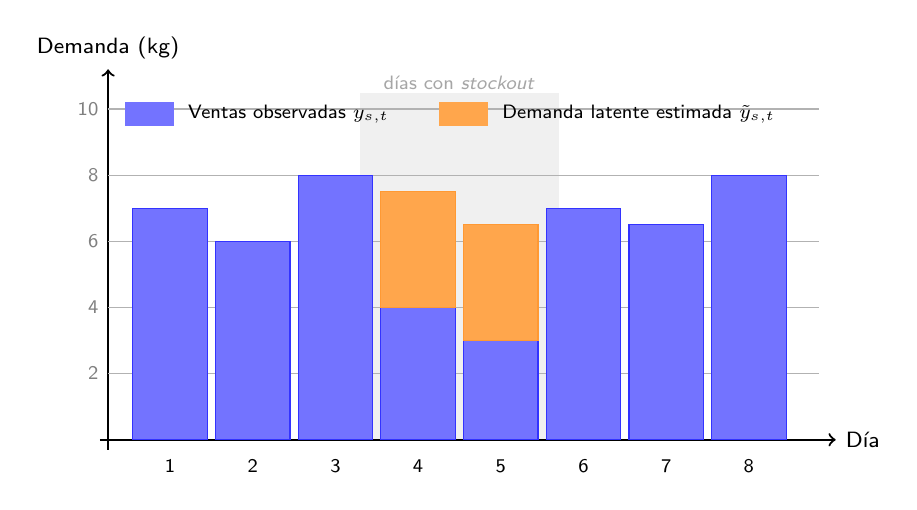
\begin{tikzpicture}[xscale=1.05, yscale=0.42]
  % Stockout background shading
  \fill[gray!12] (3.05,0) rectangle (5.45,10.5);
  % Axes
  \draw[->,thick] (-0.1,0) -- (8.8,0) node[right,font=\sffamily\footnotesize] {Día};
  \draw[->,thick] (0,-0.3) -- (0,11.2) node[above,font=\sffamily\footnotesize] {Demanda (kg)};
  \foreach \y in {2,4,6,8,10} {
    \draw[gray!60] (0,\y) -- (8.6,\y);
    \node[left,font=\sffamily\scriptsize,gray] at (0,\y) {\y};
  }
  % Day labels
  \foreach \x/\d in {0.75/1,1.75/2,2.75/3,3.75/4,4.75/5,5.75/6,6.75/7,7.75/8} {
    \node[below,font=\sffamily\scriptsize] at (\x,-0.3) {\d};
  }
  % Normal days: single blue bar
  \fill[blue!55]  (0.3,0) rectangle (1.2,7);   % day 1
  \fill[blue!55]  (1.3,0) rectangle (2.2,6);   % day 2
  \fill[blue!55]  (2.3,0) rectangle (3.2,8);   % day 3
  \fill[blue!55]  (5.3,0) rectangle (6.2,7);   % day 6
  \fill[blue!55]  (6.3,0) rectangle (7.2,6.5); % day 7
  \fill[blue!55]  (7.3,0) rectangle (8.2,8);   % day 8
  % Stockout days: blue (observed) + orange extension (latent)
  \fill[blue!55]  (3.3,0) rectangle (4.2,4);   % day 4 observed
  \fill[orange!70](3.3,4) rectangle (4.2,7.5); % day 4 latent extra
  \fill[blue!55]  (4.3,0) rectangle (5.2,3);   % day 5 observed
  \fill[orange!70](4.3,3) rectangle (5.2,6.5); % day 5 latent extra
  % Bar outlines
  \foreach \xa/\xb/\h in {0.3/1.2/7, 1.3/2.2/6, 2.3/3.2/8, 5.3/6.2/7, 6.3/7.2/6.5, 7.3/8.2/8} {
    \draw[blue!80,thin] (\xa,0) rectangle (\xb,\h);
  }
  \draw[blue!80,thin]   (3.3,0) rectangle (4.2,4);
  \draw[orange!80,thin] (3.3,4) rectangle (4.2,7.5);
  \draw[blue!80,thin]   (4.3,0) rectangle (5.2,3);
  \draw[orange!80,thin] (4.3,3) rectangle (5.2,6.5);
  % Stockout label
  \node[font=\sffamily\scriptsize,gray!70] at (4.25,10.8) {días con \textit{stockout}};
  % Legend
  \fill[blue!55]  (0.2,9.5) rectangle (0.8,10.2);
  \node[right,font=\sffamily\scriptsize] at (0.85,9.85) {Ventas observadas $y_{s,t}$};
  \fill[orange!70](4.0,9.5) rectangle (4.6,10.2);
  \node[right,font=\sffamily\scriptsize] at (4.65,9.85) {Demanda latente estimada $\tilde{y}_{s,t}$};
\end{tikzpicture}
\shorthandon{>}%
\caption[Efecto de la censura por stockout]{Efecto de la censura por stockout: en los días con rotura (fondo gris), las ventas
registradas (azul) son inferiores a la demanda real. La estimación de la demanda latente
(naranja) corrige el sesgo antes del entrenamiento.}
\label{fig:censored_demand}
\end{figure}

Para corregirlo, el sistema implementa un preprocesador dinámico que estima la demanda latente $\tilde{y}_{s,t}$ en los días afectados por roturas de stock ($h_{s,t} > 0$). Se comparan tres estrategias alternativas de imputación:

\begin{itemize}
    \item \textbf{Clipped Scaling}: Multiplica la demanda observada por un factor configurable
    $\gamma > 0$ (valor por defecto $\gamma = 1{,}2$). Para $\gamma > 1$ e $y_{s,t} > 0$
    la estimación es simplemente $\gamma \cdot y_{s,t}$; el $\max$ actúa como salvaguarda
    ante configuraciones con $\gamma \leq 1$:
    \begin{equation}
        \tilde{y}_{s,t} = \max\!\left( y_{s,t},\ y_{s,t} \cdot \gamma \right)
    \end{equation}

    \item \textbf{Media Histórica Local}: Reemplaza el valor censurado por el máximo entre
    la demanda observada y el promedio de ventas en los días libres de stockout ($\mathcal{T}_{\text{clean},s}$)
    para dicha serie temporal específica:
    \begin{equation}
        \tilde{y}_{s,t} = \max \left( y_{s,t}, \, \frac{1}{|\mathcal{T}_{\text{clean},s}|}
        \sum_{\tau \in \mathcal{T}_{\text{clean},s}} y_{s,\tau} \right)
    \end{equation}

    \item \textbf{Supervisada (LightGBM)}: Entrena un modelo LightGBM auxiliar
    $\hat{g}$ sobre los registros históricos no afectados por stockouts, que predice la
    demanda de un \textbf{día completo sin rotura}. El vector de covariables $\mathbf{x}_{s,t}^{\text{imp}}$
    incluye: identificador de serie, mes, día de la semana, día del mes, media histórica
    de días limpios de la serie como prior, e indicadores contextuales disponibles en el
    dataset (descuento, festivo, temperatura, precipitación, humedad y viento). La
    severidad de la rotura se incorpora en la \textbf{reconciliación}: sea
    $r_{s,t} = h_{s,t}/16 \in [0, 1]$ la fracción del día perdida por el stockout, la demanda
    latente se estima recomponiendo lo observado con esa fracción de lo predicho:
    \begin{equation}
        \tilde{y}_{s,t} = y_{s,t} + r_{s,t} \cdot \max\!\left( \hat{g}(\mathbf{x}_{s,t}^{\text{imp}}),\, 0 \right)
    \end{equation}
\end{itemize}

En el benchmark oficial del propio dataset \cite{freshretailnet2025} se evalúan enfoques de aprendizaje profundo (TimesNet, CSDI, SAITS) que obtienen mejores métricas de recuperación, pero a un coste computacional incompatible con un despliegue operacional ligero; las tres estrategias aquí propuestas priorizan interpretabilidad y velocidad de inferencia. La estrategia \textbf{Supervisada (LightGBM)} es la seleccionada en el sistema final, y conviene precisar sobre qué base: no por haber ganado una comparación entre las tres, que el protocolo de censura sintética no puede dirimir (Sección~\ref{sec:imputacion_censura_sintetica}), sino porque estima la corrección de forma condicional a las covariables del día en lugar de aplicar un factor fijo o el nivel medio de la serie. Lo que la evidencia empírica sí establece es que corregir la censura compensa frente a no corregirla, y esa comparación se recoge en la Sección~\ref{sec:resultados_gemelo}. Los hiperparámetros de ese regresor auxiliar son objeto de una búsqueda propia, independiente del ajuste del modelo de \textit{forecasting} y ejecutada como un modo de ejecución separado del sistema. El protocolo y las mediciones se recogen en el Anexo~\ref{anx:tuning_imputador}, pero el resultado de esa búsqueda no se queda en el anexo: el fichero de hiperparámetros que persiste es leído por el modo de experimento y por el \textit{backtest} de coste justo, de modo que forma parte de la configuración con la que se producen las cifras finales, no solo de un apéndice documental. Esa dependencia tiene un límite conocido, y el anexo documenta cómo se descubrió: la ganancia que mide la búsqueda depende del tamaño del conjunto con el que se ajusta el imputador, hasta el punto de cambiar de signo si la validación se monta de forma que ese conjunto se encoja. El protocolo vigente lo evita separando selección y validación por tiempo y aplicando esa separación como una máscara sobre el panel completo, de modo que el maestro conserva el tamaño que tiene en producción. Aun así la validez del fichero queda acotada al tamaño de ajuste con el que se obtuvo: los metadatos de la búsqueda registran esa escala, pero es una condición documentada para quien lea el artefacto, no una comprobación que el sistema haga por sí mismo al cargarlo.

\subsection{Ingeniería de Características}
\label{sec:feature_engineering}

El sistema de previsión opera sobre un panel diario de series temporales. Dado que los modelos de \textit{Gradient Boosting} no tienen memoria temporal intrínseca, la información histórica debe codificarse explícitamente como columnas del vector de entrada. El proceso de ingeniería de características transforma el panel preparado en un \textit{frame} supervisado donde cada fila representa un origen de predicción con su vector de covariables correspondiente.

Las características se organizan en cinco grupos funcionales:

\begin{enumerate}
    \item \textbf{Características Calendáricas}: Codifican la posición temporal del origen de predicción. Incluyen el día de la semana ($\in [0,6]$), el día del mes, el mes, la semana del año, un indicador binario de fin de semana, un indicador de festivo (\texttt{holiday\_flag}) y un indicador de actividad promocional especial (\texttt{activity\_flag}). Estas variables capturan la estacionalidad semanal y mensual identificada en el análisis exploratorio (véase Capítulo~\ref{chap:analisis_datos}).

    \item \textbf{Lags de Demanda y Ventanas Deslizantes}: Para capturar la autocorrelación de la serie, se calculan lags de la demanda observada en los instantes $t-1$, $t-7$ y $t-14$. La elección no es arbitraria: el análisis de la función de autocorrelación (ACF) del Capítulo~\ref{chap:analisis_datos} reveló picos significativos en los cuatro retardos múltiplos de 7 (7, 14, 21 y 28), con amplitud decreciente de 0,62 a 0,39, confirmando la estacionalidad semanal dominante del dataset. El lag $t-1$ captura inercia de corto plazo (efecto del día anterior); $t-7$ y $t-14$ recogen el ciclo semanal y quincenal, los dos de mayor autocorrelación tras el propio $t-1$; un cuarto retardo a $t-28$, que aproximaba el ciclo mensual de reposición y cuya autocorrelación seguía siendo significativa, se probó y se retiró del conjunto final: con 90 días de historia disponible su coste no está en el número de columnas sino en el arranque en frío, porque el primer origen predecible de cada serie se retrasa hasta que el retardo más largo tiene dato: 28 días en lugar de 14, lo que cuesta catorce orígenes por serie. Sobre ventanas de 7 y 14 días se calculan además la media, la suma y la desviación estándar rodantes. Todos los estadísticos se computan con desplazamiento de un día (\texttt{shift(1)}) para garantizar ausencia de \textit{data leakage}.

    \item \textbf{Lags de Variables Exógenas Externas}: Se construyen lags en los instantes $t-1$, $t-7$ y $t-14$ para la variable de descuento (\texttt{discount}) y las cuatro variables meteorológicas (temperatura, precipitación, humedad y viento). Son covariables externas al sistema de inventario que modulan la demanda sin depender del estado del stock.

    \item \textbf{Lags de Stockout}: Las horas diarias sin stock (\texttt{stockout\_hours}) se tratan como grupo propio por su doble rol en el sistema: actúan como señal proxy de la demanda latente en el módulo de imputación (Sección~\ref{sec:demanda_censurada}) y como covariable del modelo de forecasting que informa sobre la presión histórica de rotura. Se calculan lags en los mismos instantes ($t-1, t-7, t-14$) y medias rodantes a 7 y 14 días.

    \item \textbf{Identificadores Estáticos}: cada serie del panel es el par (\texttt{product\_id}, \texttt{store\_id}) definido al inicio de este bloque; junto a él se incluyen los identificadores que sitúan a ese par en la jerarquía del catálogo y de la red de tiendas -- \texttt{city\_id}, \texttt{management\_group\_id} y las tres categorías de producto --, todos como variables categóricas nativas, sin construir a mano ninguna jerarquía adicional. Cómo codifica cada \textit{backend} estas categóricas de alta cardinalidad, y por qué esa codificación pesa en la elección del campeón, se trata en la Sección~\ref{sec:eleccion_backends}.
\end{enumerate}

La Tabla~\ref{tab:features_summary} resume el número de características resultantes por grupo.

\begin{table}[htbp]
    \centering
    \small
    \setlength{\tabcolsep}{4pt}
    \begin{tabular}{lcc}
        \toprule
        \textbf{Grupo} & \textbf{N\textordmasculine{} características} & \textbf{Ejemplos} \\
        \midrule
        Calendáricas & 7 & \texttt{day\_of\_week}, \texttt{holiday\_flag}, \texttt{activity\_flag} \\
        Lags de demanda & 3 & \texttt{demand\_lag\_1}, \texttt{demand\_lag\_14} \\
        Ventanas deslizantes & 6 & \texttt{demand\_roll\_mean\_7}, \texttt{demand\_roll\_std\_14} \\
        Lags de exógenas & 15 & \texttt{discount\_lag\_7}, \texttt{avg\_temperature\_lag\_1} \\
        Lags de stockout & 5 & \texttt{stockout\_lag\_7}, \texttt{stockout\_roll\_mean\_14} \\
        Identificadores estáticos & 7 & \texttt{store\_id}, \texttt{third\_category\_id} \\
        \midrule
        \textbf{Total} & \textbf{43} & \\
        \bottomrule
    \end{tabular}
    \caption{Resumen de características del frame supervisado.}
    \label{tab:features_summary}
\end{table}

\subsection{Modelado Probabilístico: Función de Pérdida Pinball}
\label{sec:pinball}
El núcleo de la estimación probabilística de la demanda reside en la optimización directa de cuantiles. En lugar de predecir la media condicional (que asume simetría en los errores y no proporciona cotas de riesgo logístico), el sistema optimiza de forma independiente el conjunto de cuantiles objetivo mediante la función de pérdida asimétrica conocida como \textit{Pinball Loss} (o pérdida cuantílica) \cite{koenker2005quantile}.

Para un cuantil de interés $q \in (0, 1)$, la pérdida \textit{Pinball} asociada a una observación real $y$ y su predicción $\hat{y}_q$ (la cantidad en unidades físicas que el modelo predice al nivel $q$) se formula matemáticamente de dos maneras equivalentes:

\begin{equation}
    \mathcal{L}_q(y, \hat{y}_q) = \max \left( q(y - \hat{y}_q), \, (q - 1)(y - \hat{y}_q) \right)
\end{equation}

O bien, expresada en su forma condicional por tramos para enfatizar la asimetría:

\begin{equation}
    \mathcal{L}_q(y, \hat{y}_q) =
    \begin{cases}
        q \cdot (y - \hat{y}_q) & \text{si } y \ge \hat{y}_q \quad \text{(subestimación)} \\
        (1 - q) \cdot (\hat{y}_q - y) & \text{si } y < \hat{y}_q \quad \text{(sobreestimación)}
    \end{cases}
\end{equation}

Por ejemplo, para $q = 0{,}9$ y una demanda real $y = 10$ kg: si el modelo predice $\hat{y}_q = 8$ kg (subestimación), la pérdida es $0{,}9 \cdot (10 - 8) = 1{,}8$; si predice $\hat{y}_q = 12$ kg (sobreestimación), es $0{,}1 \cdot (12 - 10) = 0{,}2$. La penalización por subestimar es nueve veces mayor, lo que incentiva al modelo a situarse en el percentil 90 de la demanda. La Figura~\ref{fig:pinball_asymmetry} ilustra gráficamente esta asimetría para los dos cuantiles extremos.

\begin{figure}[H]
\centering
\shorthandoff{>}%
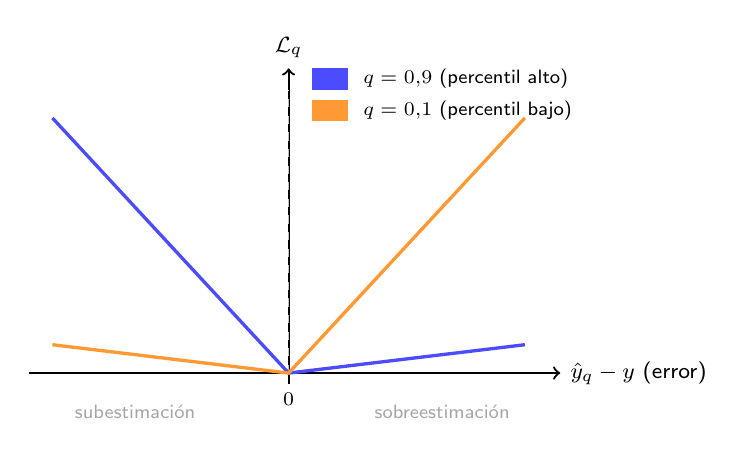
\begin{tikzpicture}[xscale=0.75, yscale=0.9]
  % Axes
  \draw[->,thick] (-4.4,0) -- (4.6,0) node[right,font=\sffamily\footnotesize] {$\hat{y}_q - y$ (error)};
  \draw[->,thick] (0,-0.15) -- (0,4.3) node[above,font=\sffamily\footnotesize] {$\mathcal{L}_q$};
  % Zero label
  \node[below,font=\sffamily\scriptsize] at (0,-0.15) {$0$};
  % Dashed vertical
  \draw[dashed,gray!50] (0,0) -- (0,4.0);
  % q=0.9: slope 0.9 left (steep), slope 0.1 right (flat)
  \draw[blue!70,very thick] (-4,3.6) -- (0,0) -- (4,0.4);
  % q=0.1: slope 0.1 left (flat), slope 0.9 right (steep)
  \draw[orange!80,very thick] (-4,0.4) -- (0,0) -- (4,3.6);
  % Region labels
  \node[font=\sffamily\scriptsize,gray!70] at (-2.6,-0.55) {subestimación};
  \node[font=\sffamily\scriptsize,gray!70] at (2.6,-0.55) {sobreestimación};
  % Legend — placed right of y-axis, top area (clear of both arms)
  \fill[blue!70]   (0.4,4.0) rectangle (1.0,4.3);
  \node[right,font=\sffamily\scriptsize] at (1.1,4.15) {$q=0{,}9$ (percentil alto)};
  \fill[orange!80] (0.4,3.55) rectangle (1.0,3.85);
  \node[right,font=\sffamily\scriptsize] at (1.1,3.70) {$q=0{,}1$ (percentil bajo)};
\end{tikzpicture}
\shorthandon{>}%
\caption[Asimetría de la pérdida \textit{pinball}]{Asimetría de la función de pérdida \textit{pinball} para dos cuantiles extremos.
Para $q=0{,}9$ (azul), subestimar la demanda se penaliza nueve veces más que sobreestimarla,
empujando las predicciones hacia valores altos. Para $q=0{,}1$ (naranja), el efecto es inverso.}
\label{fig:pinball_asymmetry}
\end{figure}

La minimización de la pérdida esperada bajo $\mathcal{L}_q$ tiene como solución óptima el cuantil $q$ de la distribución de la demanda:

\begin{equation}
    \arg\min_{\hat{y}_q} \mathbb{E}_{Y} \left[ \mathcal{L}_q(Y, \hat{y}_q) \right] = F_{Y}^{-1}(q)
\end{equation}

donde $F_Y^{-1}(q)$ es el cuantil $q$ de la demanda: el valor por debajo del cual cae el
$q \cdot 100\%$ de las observaciones históricas.

\begin{center}
\fbox{\begin{minipage}{0.88\textwidth}
\textbf{Nexo metodológico: Pinball Loss $\leftrightarrow$ Newsvendor.}\\[4pt]
El modelo del \textit{Newsvendor} \cite{silver1998inventory} demuestra que el nivel de cobertura óptimo bajo costes asimétricos viene determinado por el \textit{fractil crítico}:
$$q^\star = \frac{c_u}{c_u + c_o}$$
donde $c_u$ es el coste por unidad no servida (rotura de stock) y $c_o$ el coste por unidad sobrante, siendo la cantidad óptima de pedido el cuantil de demanda correspondiente $O^\star = F_Y^{-1}(q^\star)$. Este es exactamente el cuantil que minimiza la Pinball Loss. Por tanto, \textbf{entrenar el modelo con Pinball en $q = q^\star$ es equivalente a optimizar directamente la política de pedido}, sin ninguna etapa de postproceso adicional. Esto diferencia al sistema de los enfoques que predicen la media y después aplican un nivel de servicio fijo: aquí la decisión de inventario está integrada en el proceso de entrenamiento.
\end{minipage}}
\end{center}

En la formulación general, el modelo minimiza la pérdida esperada de forma conjunta sobre todas las series $s \in \mathcal{S}$ y todos los instantes de decisión $t \in \mathcal{T}$:

\begin{equation}
    \hat{\theta} = \arg\min_{\theta}
    \frac{1}{|\mathcal{S}||\mathcal{T}|}
    \sum_{s \in \mathcal{S}} \sum_{t \in \mathcal{T}}
    \mathcal{L}_{q_s^*}\!\left(Y_{s,t},\; f_\theta(\mathbf{x}_{s,t})\right)
    \label{eq:training_objective}
\end{equation}

donde $q_s^*$ representa el fractil crítico específico de la serie $s$ en función de sus márgenes comerciales y costes de merma individuales. En un entorno productivo con contabilidad analítica por referencia, este fractil variará por producto; no obstante, al no disponer en el conjunto de datos de partida de los costes desglosados por SKU, el sistema evalúa de manera homogénea una política de catálogo canónica (como se detalla y justifica en la Sección~\ref{sec:cost_profiles}).

Al entrenar con RMSE o MAE se minimiza el error estadístico pero no el coste logístico, lo que es inconsistente con el objetivo operativo del sistema. Por eso el objetivo de la Ecuación~\ref{eq:training_objective}, orientado al cuantil que dicta el coste, es el pilar central de la arquitectura. Para resolver eficientemente este problema de optimización no diferenciable por tramos, la siguiente subsección examina las implementaciones de \textit{Gradient Boosting} seleccionadas.

\subsection{Selección de las Implementaciones de Boosting}
\label{sec:eleccion_backends}

De las tres implementaciones de referencia revisadas en el Estado del Arte, el sistema implementa y compara empíricamente \textbf{dos}: LightGBM y CatBoost, descartando XGBoost antes de la fase experimental por motivos de alcance y redundancia metodológica:

\begin{itemize}
    \item \textbf{Descarte razonado de XGBoost:} Aunque desde su versión 1.5 XGBoost soporta particionamiento categórico nativo sin requerir \textit{one-hot encoding}, comparte con LightGBM el mismo principio algorítmico: ordenar las categorías mediante el estadístico del gradiente. Incorporar un tercer motor con idéntica lógica de partición duplicaría el coste computacional del protocolo de \textit{backtesting} sin aportar un contraste metodológico real.
    \item \textbf{Ortogonalidad de CatBoost:} Es la única de las tres librerías que introduce un mecanismo conceptualmente diferenciado: los \textit{Ordered Target Statistics}, que proporcionan una defensa matemática explícita frente a la fuga de información (\textit{target leakage}) en identificadores de alta cardinalidad (como los 500 SKUs del catálogo), y los árboles simétricos (\textit{oblivious trees}), que actúan como regularizadores estructurales en series con historial temporal corto.
    \item \textbf{Criterio de selección y paridad experimental:} La elección final del modelo campeón \textbf{no se basa en preferencias teóricas de diseño, sino en los resultados empíricos} del protocolo de evaluación (Sección~\ref{sec:promocion}). Esta distinción es crucial, ya que el orden de rendimiento según error puntual (RMSE) no coincide necesariamente con el orden según coste de inventario real. Asimismo, para garantizar una comparación en estricta igualdad de condiciones, la estimación nativa de incertidumbre de CatBoost no se utiliza: ambos motores operan bajo el mismo envoltorio multi-cuantil y la misma capa de calibración Conformal.
\end{itemize}

\subsection{Arquitectura Multi-Modelo y Corrección del Quantile Crossing}
\label{sec:crossing}
Dado que los frameworks estándar de Gradient Boosting están diseñados para optimizar un único objetivo escalar por modelo, el sistema implementa un \textbf{Wrapper Cuantílico Multi-Modelo}. Este componente instancia y entrena de forma independiente $M$ estimadores, cada uno sintonizado para un cuantil específico del conjunto $\mathcal{Q} = \{q_1, q_2, \dots, q_M\}$, donde $q_1 < q_2 < \dots < q_M$.

\paragraph{El estimador puntual se ajusta en el fractil crítico.} Junto a esos $M$ estimadores, el envoltorio ajusta un modelo adicional cuya salida es la \emph{predicción puntual} $\hat{y}$ del sistema. Ese modelo no se entrena contra el error cuadrático ni contra el absoluto, sino con la misma \textit{pinball loss} evaluada en el fractil crítico del \textit{Newsvendor} ($\tau = q^\star = 0{,}80$ con la estructura de costes de este trabajo), de forma coherente con el argumento de la Sección~\ref{sec:pinball}: entrenar contra RMSE o MAE optimizaría una magnitud que no es la que gobierna la decisión. Ambos motores lo hacen de forma equivalente, mediante \texttt{Quantile:alpha} en CatBoost y el objetivo \texttt{quantile} en LightGBM.

Esta elección tiene una consecuencia que conviene anticipar aquí, porque condiciona la lectura de los resultados del Capítulo~\ref{chap:resultados}: $\hat{y}$ \textbf{no aspira a estimar la mediana ni la media condicional}, sino un cuantil alto de la distribución. Toda métrica de error puntual calculada sobre él (el MAE y el RMSE que reporta la Tabla~\ref{tab:metrics_predictive}) mide, por tanto, un estimador distinto del que esas métricas premian, y su comparación con la de un predictor central está sesgada de antemano.

Conviene además separar el objetivo de entrenamiento de la calibración efectivamente alcanzada. Que la pérdida se evalúe en $\tau = 0{,}80$ fija hacia dónde se optimiza, no garantiza que la cobertura empírica fuera de muestra sea esa: el Capítulo~\ref{chap:resultados} documenta que no lo es. El estimador puntual queda por añadidura fuera de la corrección conformal, que actúa sobre los extremos del intervalo y no sobre él, y esas dos razones juntas son las que impiden tomar de él la cantidad de pedido, que se obtiene de la rejilla calibrada (Sección~\ref{sec:newsvendor_operativo}).

\paragraph{El fenómeno del \textit{Quantile Crossing}.}
Al entrenarse cada estimador sin comunicación con los demás, esta arquitectura introduce el riesgo de \textbf{cruzamiento de cuantiles} (\textit{quantile crossing}) \cite{koenker2005quantile}: una patología en la que, para una observación concreta, el modelo de un cuantil inferior predice un valor mayor que el de un cuantil superior (por ejemplo, $\hat{y}_{0{,}7} > \hat{y}_{0{,}9}$), violando la monotonicidad axiomática de las funciones de distribución acumulada.

\paragraph{Corrección mediante \textit{Rearrangement} de Chernozhukov.}
Para restaurar la monotonicidad sin distorsionar las estimaciones, el sistema aplica el \textbf{\textit{rearrangement}} propuesto por Chernozhukov et al. \cite{chernozhukov2010quantile}. Dado el vector de predicciones crudas $\tilde{\mathbf{y}}_{s,t} = (\tilde{y}_{s,t}^{(1)}, \dots, \tilde{y}_{s,t}^{(M)})$, el método consiste en reordenar sus componentes en orden no decreciente:

\begin{equation}
    \hat{\mathbf{y}}_{s,t} = \text{sort}\!\left(\tilde{\mathbf{y}}_{s,t}\right)
\end{equation}

Esta operación garantiza formalmente la monotonicidad de la rejilla estimada:

\begin{equation}
    \hat{y}_{s,t}^{(1)} \le \hat{y}_{s,t}^{(2)} \le \dots \le \hat{y}_{s,t}^{(M)}
\end{equation}

Este procedimiento es computacionalmente ligero ($\mathcal{O}(M \log M)$, equivalente a ordenar con \texttt{np.sort} sobre el eje de cuantiles) y posee una propiedad teórica fundamental \cite{chernozhukov2010quantile}: el \textit{rearrangement} reduce (o mantiene) la pérdida cuantílica integrada sobre todos los niveles de cuantil respecto a las estimaciones originales.

\paragraph{Descarte de la Regresión Isotónica (PAVA).}
Frente al \textit{rearrangement}, la alternativa clásica para forzar monotonicidad es la regresión isotónica mediante el algoritmo \textbf{PAVA} (\textit{Pool Adjacent Violators Algorithm}) \cite{barlow1972isotonic}. PAVA recorre el vector y promedia sucesivamente los pares adyacentes que violan el orden para encontrar la proyección más cercana en norma $L_2$. Sin embargo, PAVA no ofrece garantías de mejora sobre la función de pérdida \textit{Pinball} y modifica activamente los valores predichos al promediarlos, mientras que el \textit{rearrangement} preserva exactamente los cuantiles aprendidos por el modelo reorganizando únicamente sus posiciones.

\subsection{Sintonización Biobjetivo y Frente de Pareto: Coste Logístico vs. Winkler Score}
\label{sec:tuning_metodologia}
\label{sec:pareto}

Históricamente, los sistemas de predicción de demanda sintonizan sus hiperparámetros minimizando funciones de error simétrico promedio (como el MAE o el RMSE). Sin embargo, en un entorno de inventario con costes fuertemente asimétricos, una mejora en el error cuadrático medio no se traduce necesariamente en una reducción de los costes operativos reales, y optimizar un único cuantil aislado puede deformar la dispersión del resto de la distribución predicha.

Para resolver este compromiso, el sistema implementa una \textbf{Búsqueda de Hiperparámetros Biobjetivo} utilizando \textit{Optuna} \cite{akiba2019optuna} y el algoritmo TPE multiobjetivo multivariante (\textit{Tree-structured Parzen Estimator}). En cada iteración, el optimizador evalúa simultáneamente dos objetivos en conflicto sobre la ventana de evaluación calibrada conformalmente:

\begin{enumerate}
    \item \textbf{Objetivo 1 (Coste Logístico de Inventario):} Evalúa el coste económico total del modelo \textit{Newsvendor} ($c_u \cdot \text{rotura} + c_o \cdot \text{exceso}$) inducido por la decisión de compra en el fractil crítico.
    \item \textbf{Objetivo 2 (Calidad de la Incertidumbre - Winkler Score):} Evalúa la nitidez y cobertura del intervalo central $[P10, P90]$ mediante la regla de puntuación estrictamente propia definida a continuación.
\end{enumerate}

Esta formulación produce una \textbf{Frontera de Pareto empírica} que identifica las configuraciones no dominadas (aquellas donde es imposible reducir el coste logístico sin degradar la fiabilidad de las bandas de incertidumbre). El sistema selecciona el candidato óptimo de la frontera y lo somete al protocolo de validación temporal.

\paragraph{Protocolo de Doble Ventana Temporal y Puerta de Validación.}
Para evitar que el optimizador sobreajuste los hiperparámetros a una ventana temporal específica, la búsqueda se estructura en un protocolo estricto de dos etapas desacopladas:

\begin{enumerate}
    \item \textbf{Ventana de Selección ($N=30$ extracciones temporales):} Optuna explora el espacio de búsqueda biobjetivo sobre un conjunto histórico cerrado, construyendo la frontera de Pareto de candidatos.
    \item \textbf{Ventana de Validación \textit{Out-of-Sample} ($N=25$ extracciones independientes posteriores):} La configuración seleccionada en la frontera de Pareto no se adopta automáticamente. Se somete a una \textbf{puerta de validación} donde compite contra los hiperparámetros por defecto sobre una ventana temporal futura genuinamente no observada. Se calcula un intervalo de confianza \textit{bootstrap} al 95\% sobre la diferencia pareada de costes: solo si la mejora es estadísticamente significativa ($\text{IC}_{95\%}^{\text{sup}} < 0$), los nuevos parámetros son persistidos en \texttt{models/forecasting\_params.json} para su uso en el \textit{backtesting} global.
\end{enumerate}

\subsubsection{Evaluación de la Calidad de los Intervalos: Winkler Score}
\label{sec:winkler}
El \textbf{Winkler Score} \cite{winkler1972scoring} es una regla de puntuación estrictamente propia que penaliza simultáneamente la amplitud del intervalo (\textit{nitidez}) y los fallos de cobertura en una única métrica consolidada.

Para un intervalo central $[L_{s,t},\, U_{s,t}]$ con nivel de significancia nominal $\alpha$ ($\alpha = 0{,}2$ para el intervalo central P10--P90, que deja fuera el $10\%$ en cada cola):

\begin{equation}
    W(L, U, y) = \begin{cases}
        (U_{s,t} - L_{s,t}) & \text{si } L_{s,t} \le y_{s,t} \le U_{s,t} \\[4pt]
        (U_{s,t} - L_{s,t}) + \dfrac{2}{\alpha}(L_{s,t} - y_{s,t})
        & \text{si } y_{s,t} < L_{s,t} \\[4pt]
        (U_{s,t} - L_{s,t}) + \dfrac{2}{\alpha}(y_{s,t} - U_{s,t})
        & \text{si } y_{s,t} > U_{s,t}
    \end{cases}
\end{equation}

El primer término representa el \emph{pago base} correspondiente a la amplitud del intervalo $(U - L)$, incentivando bandas estrechas. Cuando la demanda real $y_{s,t}$ cae fuera del intervalo, se añade una penalización lineal a la distancia al borde multiplicada por el factor $2/\alpha$ (en este caso, un factor amplificador de $\times 10$). La métrica se promedia sobre todas las series y horizontes evaluados (\textbf{valores más bajos indican mejor calibración}).

\medskip
\noindent\textbf{Ejemplo numérico.} Supóngase que el modelo predice el intervalo $[10, 20]$ unidades para la demanda acumulada (amplitud $= 10$, $\alpha = 0{,}2$):

\begin{itemize}
    \item \textbf{Caso 1 (acierto):} si la demanda real es $y = 15$ (dentro del intervalo), $W = 20 - 10 = \mathbf{10}$. Solo se penaliza la amplitud.
    \item \textbf{Caso 2 (fallo por defecto):} si la demanda real es $y = 5$ ($y < L$), $W = 10 + \frac{2}{0{,}2}(10 - 5) = 10 + 50 = \mathbf{60}$. El fallo de cobertura multiplica por seis la penalización.
    \item \textbf{Caso 3 (fallo por exceso):} si la demanda real es $y = 25$ ($y > U$), $W = 10 + \frac{2}{0{,}2}(25 - 20) = 10 + 50 = \mathbf{60}$.
\end{itemize}

Si en cambio el modelo produjera un intervalo trivial e hiper-conservador $[0, 100]$ unidades, cubriría siempre la demanda real pero incurriría en un pago constante de $W = 100$, muy superior al del intervalo ajustado. Por estas propiedades, el \textbf{Winkler Score se integra directamente como el segundo objetivo en la búsqueda biobjetivo}: actúa penalizando activamente aquellas configuraciones de hiperparámetros que logren reducir el coste logístico a expensas de deformar, ensanchar o descalibrar los intervalos de incertidumbre predichos.

\subsection{Calibración: Mondrian Conformal Prediction}
\label{sec:conformal}
El modelo entrenado con \textit{Pinball Loss} en $q = 0{,}9$ debería, en teoría, producir
predicciones que la demanda real supere solo el 10\% de las veces. En la práctica esto no
está garantizado: el modelo puede estar sistemáticamente sesgado, haber sobreajustado, o
simplemente no haber visto suficientes muestras de ciertos SKUs. La calibración conformal
resuelve este problema de forma agnóstica al modelo: ajusta los intervalos \textit{a
posteriori} para que la cobertura empírica sobre un conjunto de holdout genuinamente no
visto sea exactamente $(1-\alpha)$, con garantía finita y sin supuestos sobre la
distribución de la demanda.

El sistema utiliza \textbf{Split Conformal Prediction} \cite{angelopoulos2021gentle} como
mecanismo de calibración: tras entrenar el modelo, se reserva un subconjunto de calibración
sobre el que se calculan los errores de cobertura; a partir de ellos se obtiene un factor
corrector $\hat{q}$ que, aplicado en predicción, garantiza que el $(1-\alpha)\cdot 100\%$ de
las observaciones futuras caigan dentro del intervalo.

La garantía de un $\hat{q}$ global es de cobertura \textbf{marginal}: el 80\% de cobertura
se cumple \textit{en media sobre todo el catálogo}, pero puede enmascarar desigualdades
críticas por familia de producto: el modelo podría cubrir el 90\% de los productos
estables y solo el 70\% de los intermitentes, y la media seguiría siendo 80\%.

Para obtener cobertura \textbf{condicional por categoría}, el sistema extiende Split CP
con la estrategia \textbf{Mondrian} \cite{vovk2005algorithmic}: en lugar de un único
$\hat{q}$ global, se calcula un $\hat{q}_g$ independiente para cada grupo taxonómico $g$,
garantizando que la cobertura se cumpla dentro de cada familia de producto por separado.
El $\hat{q}$ global se conserva como valor de seguridad (\textit{fallback}) para SKUs cuya
categoría no haya aparecido en el set de calibración. El procedimiento completo es el
siguiente:

\begin{enumerate}
    \item \textbf{Partición Taxonómica}: Las series temporales se agrupan en categorías homogéneas
    mediante su identificador jerárquico \texttt{third\_category\_id}, asegurando que la
    calibración refleje el comportamiento propio de cada familia de productos.

    \item \textbf{Score de No-Conformidad Local (CQR)}: Para cada observación $i$ en el conjunto
    de calibración $\mathcal{I}_{\text{cal}}$, se calcula la puntuación de no-conformidad
    siguiendo el método \textit{Conformalized Quantile Regression} \cite{romano2019conformalized}.
    Dado que el sistema siempre produce predicciones cuantílicas (sección~\ref{sec:pinball}),
    el score mide cuánto se desvía la observación real de los extremos del intervalo predicho:
    \begin{equation}
        s_i = \max \left( \hat{y}_{\alpha/2}(x_i) - y_i, \;
        y_i - \hat{y}_{1-\alpha/2}(x_i) \right)
    \end{equation}
    donde $\hat{y}_{\alpha/2}$ y $\hat{y}_{1-\alpha/2}$ son las predicciones en los cuantiles
    inferior y superior del intervalo. Si $y_i$ cae dentro del intervalo, $s_i < 0$; si cae
    fuera, $s_i > 0$ y mide la distancia al borde más cercano.

    \textit{Ejemplo}: si el modelo predice el intervalo $[8, 14]$ kg y la demanda real es
    17 kg, el score es $s_i = 17 - 14 = 3$ (la demanda superó el límite superior por 3 kg).
    Si la demanda real fuera 11 kg (dentro del intervalo), el score sería negativo y no se
    penalizaría. El $\hat{q}_g$ del paso siguiente recoge cuánto hay que ensanchar el
    intervalo para que este tipo de fallos no supere el $\alpha\%$ de las veces.

    \item \textbf{Factor de Corrección por Categoría y Salvaguarda Global}: Para cada grupo taxonómico $g$, se recopila el subconjunto de scores locales $\mathcal{S}_g = \{s_i : \text{SKU}_i \in g\}$ y se ordenan de forma no decreciente $s_{g,(1)} \le s_{g,(2)} \le \dots \le s_{g,(n_g)}$ donde $n_g = |\mathcal{S}_g|$. El factor de corrección $\hat{q}_g$ se calcula determinando la posición del estadístico de orden con corrección de muestra finita:
    \begin{equation}
        k_g = \min\left( \left\lceil (n_g + 1)(1 - \alpha) \right\rceil,\; n_g \right), \qquad \hat{q}_g = \max\left( s_{g,(k_g)},\; 0 \right)
    \end{equation}
    Si una categoría no cuenta con observaciones en la ventana de calibración ($n_g = 0$) o aparece por primera vez durante la inferencia, el sistema recurre automáticamente al factor de corrección global $\hat{q}_{\text{global}}$ calculado sobre la totalidad de $\mathcal{I}_{\text{cal}}$ como salvaguarda (\textit{fallback}).

    \item \textbf{Ajuste Simétrico y Traslación Operativa al Fractil Crítico}: En inferencia, el factor corrector $\hat{q}_g$ se aplica simétricamente a los cuantiles periféricos acotando el límite inferior en cero para evitar predicciones físicas imposibles:
    \begin{equation}
        \hat{y}_{q}^{\,\text{adj}}(x) =
        \begin{cases}
            \max\!\left(\hat{y}_q(x) - \hat{q}_g,\; 0\right) & \text{si } q < 0{,}5 \\
            \hat{y}_q(x) & \text{si } q = 0{,}5 \\
            \max\!\left(\hat{y}_q(x) + \hat{q}_g,\; 0\right) & \text{si } q > 0{,}5
        \end{cases}
    \end{equation}
    Este ensanchamiento produce bandas con cobertura condicional garantizada dentro de cada grupo y, simultáneamente, traslada una ventaja directa a la operativa de compras: al calcular la cantidad de pedido $O_{s,t}$ interpolando en el fractil crítico ($q^\star = 0{,}80$) entre la mediana y el cuantil superior $P90$ calibrado (Sección~\ref{sec:newsvendor_operativo}), la orden se incrementa proporcionalmente en $+0{,}75 \cdot \hat{q}_g$. Esto genera automáticamente un \textbf{colchón de stock de seguridad adaptativo por categoría} que protege al almacén contra el coste asimétrico de rotura ($c_u = 4{,}0$ frente a $c_o = 1{,}0$) en función de la verdadera dispersión empírica de cada familia de productos.
\end{enumerate}

\paragraph{Limitación: intercambiabilidad en series temporales.}
La garantía de cobertura de Split CP y CQR asume que las observaciones de calibración y test son
intercambiables, es decir, que su distribución conjunta es invariante a permutaciones. Esta
propiedad no se cumple en series temporales con dependencia temporal o no-estacionariedad: los
residuos de calibración (últimos días del split de entrenamiento) pueden no ser representativos
del comportamiento del periodo de evaluación. Las implicaciones empíricas de esta limitación
se discuten en la Sección~\ref{sec:resultados_conformal}. Conviene precisar que el incumplimiento
del supuesto no anula la garantía sino que la degrada de forma acotada en función de la magnitud de
la desviación \cite{barber2023beyond}; los algoritmos que lo relajan explícitamente
(como EnbPI \cite{xu2021conformal} o ACI \cite{gibbs2021adaptive}, comparados empíricamente sobre
series de demanda por Zaffran et al.\ \cite{zaffran2022adaptive}) quedan como línea de trabajo futuro.

\subsubsection{Métricas de Evaluación de Intervalos de Confianza}
Para evaluar la calidad de los intervalos de confianza generados por la capa conformal,
se emplean dos métricas complementarias al Winkler Score (definido en la Sección~\ref{sec:winkler}):

\begin{itemize}
    \item \textbf{PICP (Prediction Interval Coverage Probability)}: Mide simplemente
    qué fracción de las observaciones reales cayó dentro del intervalo predicho:
    \begin{equation}
        \text{PICP} = \frac{1}{N} \sum_{i=1}^N \mathbb{I} \left( L_i \le y_i \le U_i \right)
    \end{equation}
    Donde $\mathbb{I}(\cdot)$ vale 1 si la condición se cumple y 0 si no.
    Con cuantiles P10--P90, la cobertura teórica garantizada por Predicción Conformal es
    $1 - \alpha = 0{,}80$. Un PICP de 0,78 significaría que el intervalo contiene el valor
    real el 78\% de las veces, prácticamente lo prometido. Un PICP muy inferior a 0,80
    indica infracobertura (el modelo es demasiado confiado); muy superior indica
    supercobertura (intervalos excesivamente conservadores).

    \item \textbf{MPIW (Mean Prediction Interval Width)}: Mide la amplitud media de los
    intervalos:
    \begin{equation}
        \text{MPIW} = \frac{1}{N} \sum_{i=1}^N (U_i - L_i)
    \end{equation}
    Un MPIW bajo significa que el modelo predice con precisión (intervalos estrechos).
    Siempre debe leerse junto al PICP: un modelo que prediga siempre $[0, +\infty)$
    obtendría PICP $= 1{,}0$ perfecto pero MPIW infinito; un modelo que prediga
    un único valor obtendría MPIW $= 0$ pero PICP $\approx 0$. El Winkler Score
    integra ambas dimensiones en una sola métrica de optimización.
\end{itemize}

\subsection{Protocolo de Evaluación: Backtesting Walk-Forward}
\label{sec:backtesting}

La evaluación de modelos de series temporales requiere respetar el orden cronológico de los datos. La validación cruzada estándar (\textit{k-fold}) mezclaría observaciones futuras con pasadas, introduciendo \textit{data leakage} y produciendo estimaciones de rendimiento optimistas e irreales.

El sistema implementa un \textbf{backtesting walk-forward} con $K=3$ folds temporales. En cada fold, el modelo se entrena sobre datos anteriores a una fecha de corte $t_k$ y se evalúa sobre el horizonte inmediatamente posterior. Entre ambos conjuntos se interpone un \textbf{intervalo de guarda} (\textit{gap}) de exactamente $H$ días:

\begin{equation}
    \text{Fold}_k: \quad \text{Train} = \{t \leq t_k - H\}, \quad
    \underbrace{\{t_k - H < t < t_k\}}_{\text{gap}}, \quad
    \text{Test} = \{t_k \leq t < t_k + H\}
\end{equation}

donde $H = 7$ días es el horizonte de planificación. El \textit{gap} no es un detalle de implementación, sino una condición necesaria de este diseño: dado que la etiqueta $Y_{s,t}$ es la demanda \emph{acumulada} de los $H$ días siguientes a $t$ (Sección~\ref{sec:pinball}), un origen de predicción situado a menos de $H$ días del corte tendría su etiqueta parcialmente solapada con el periodo de test. Al retroceder la última fecha de entrenamiento en $H$ días se garantiza que ninguna etiqueta de entrenamiento contiene información del periodo evaluado. Esta invariante se verifica automáticamente en la batería de tests anti-\textit{data leakage} descrita en la Sección~\ref{sec:testing}.

El sistema utiliza una estrategia de \textbf{ventana de entrenamiento expansiva} (expanding window), donde todos los folds comienzan al inicio del histórico y su fecha de finalización se desplaza progresivamente. La calibración conformal descrita en la sección anterior se realiza sobre una ventana fija correspondiente a los últimos $14$ días de cada conjunto de entrenamiento (por tanto, anteriores al \textit{gap}), la cual actúa como conjunto de holdout para calcular los scores de no-conformidad sin contaminar el ajuste del modelo base. La Figura~\ref{fig:backtesting_walkforward} ilustra la estructura de los tres folds.

\begin{figure}[H]
\centering
\shorthandoff{>}%
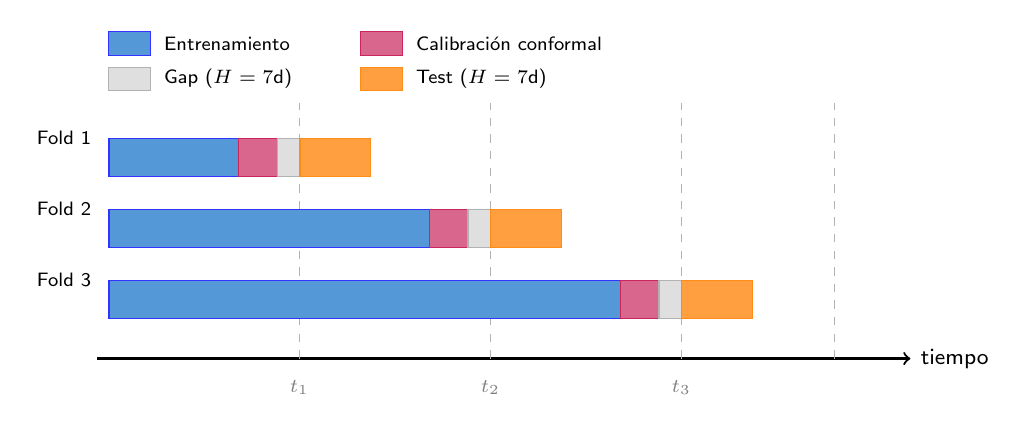
\begin{tikzpicture}[xscale=0.97, yscale=1.0,
    train/.style={fill=cyan!60!blue!70, draw=blue!80, minimum height=0.48cm},
    calib/.style={fill=purple!60, draw=purple!85, minimum height=0.48cm},
    gap/.style={fill=gray!25, draw=gray!60, minimum height=0.48cm},
    test/.style={fill=orange!75, draw=orange!90, minimum height=0.48cm},
    fold/.style={font=\sffamily\scriptsize, anchor=east}]
  % Time axis
  \draw[->,thick] (-0.15,0.1) -- (10.5,0.1) node[right,font=\sffamily\footnotesize] {tiempo};
  % Tick marks at t1,t2,t3,end
  \foreach \x/\lab in {2.5/$t_1$, 5.0/$t_2$, 7.5/$t_3$, 9.5/} {
    \draw[gray!60,dashed] (\x,0.1) -- (\x,3.35);
    \ifx\lab\empty\else \node[below,font=\sffamily\scriptsize,gray] at (\x,-0.05) {\lab}; \fi
  }
  % Fold 1
  \node[fold] at (-0.1,2.9) {Fold 1};
  \node[train, minimum width=1.7cm, anchor=west] at (0.0,2.65) {};
  \node[calib, minimum width=0.5cm, anchor=west] at (1.7,2.65) {};
  \node[gap,   minimum width=0.3cm, anchor=west] at (2.2,2.65) {};
  \node[test,  minimum width=0.9cm, anchor=west] at (2.5,2.65) {};
  % Fold 2
  \node[fold] at (-0.1,2.0) {Fold 2};
  \node[train, minimum width=4.2cm, anchor=west] at (0.0,1.75) {};
  \node[calib, minimum width=0.5cm, anchor=west] at (4.2,1.75) {};
  \node[gap,   minimum width=0.3cm, anchor=west] at (4.7,1.75) {};
  \node[test,  minimum width=0.9cm, anchor=west] at (5.0,1.75) {};
  % Fold 3
  \node[fold] at (-0.1,1.1) {Fold 3};
  \node[train, minimum width=6.7cm, anchor=west] at (0.0,0.85) {};
  \node[calib, minimum width=0.5cm, anchor=west] at (6.7,0.85) {};
  \node[gap,   minimum width=0.3cm, anchor=west] at (7.2,0.85) {};
  \node[test,  minimum width=0.9cm, anchor=west] at (7.5,0.85) {};
  % Legend (two rows)
  \fill[cyan!60!blue!70] (0.0,3.95) rectangle (0.55,4.25); \draw[blue!80] (0.0,3.95) rectangle (0.55,4.25);
  \node[right,font=\sffamily\scriptsize] at (0.6,4.10) {Entrenamiento};
  \fill[purple!60] (3.3,3.95) rectangle (3.85,4.25); \draw[purple!85] (3.3,3.95) rectangle (3.85,4.25);
  \node[right,font=\sffamily\scriptsize] at (3.9,4.10) {Calibración conformal};
  \fill[gray!25] (0.0,3.50) rectangle (0.55,3.80); \draw[gray!60] (0.0,3.50) rectangle (0.55,3.80);
  \node[right,font=\sffamily\scriptsize] at (0.6,3.65) {Gap ($H=7$d)};
  \fill[orange!75] (3.3,3.50) rectangle (3.85,3.80); \draw[orange!90] (3.3,3.50) rectangle (3.85,3.80);
  \node[right,font=\sffamily\scriptsize] at (3.9,3.65) {Test ($H=7$d)};
\end{tikzpicture}
\shorthandon{>}%
\caption[Esquema del \textit{backtesting walk-forward}]{Esquema del \textit{backtesting walk-forward} con $K=3$ folds temporales. El conjunto
de entrenamiento (azul) se expande progresivamente con cada fold; los últimos 14 días de cada ventana
de entrenamiento se reservan como calibración conformal (violeta); un intervalo de guarda de $H$ días
(gris) separa el entrenamiento del test para impedir que la etiqueta acumulada del último origen de
predicción solape con el periodo evaluado; la evaluación se realiza sobre los 7 días siguientes al
corte $t_k$ (naranja).}
\label{fig:backtesting_walkforward}
\end{figure}

El modelo \textbf{baseline} de referencia es el \textit{Seasonal Naïve}: para cada serie y fecha de predicción, replica la demanda observada en el mismo día de la semana hace 7 días. Este baseline es el más exigente en contextos con estacionalidad semanal fuerte (como el confirmado en el análisis de autocorrelación y estacionalidad de la Sección~\ref{sec:eda_temporal}, Figura~\ref{fig:eda_acf_demand}) y es el estándar de comparación utilizado en la competición M5 \cite{makridakis2022m5}. Un modelo probabilístico o de aprendizaje automático que no supere al \textit{Seasonal Naïve} en coste logístico o en error relativo (\textit{RelMAE}) no aporta valor operativo frente a una heurística determinista trivial.

\subsubsection{Variación de los Targets de Validación por Estrategia}

Es importante destacar un detalle del protocolo de evaluación predictiva cuando se comparan diferentes estrategias de tratamiento de la censura. Bajo el flujo de validación convencional del backtesting walk-forward:
\begin{itemize}
    \item Para la estrategia sin corrección (\textit{Observed}), la variable objetivo en validación ($y_{\text{true}}$) son las ventas reales registradas.
    \item Para las estrategias con corrección (\textit{Latent}), la variable objetivo en validación es la demanda ya imputada (por ejemplo, mediante el estimador supervisado de la Sección~\ref{sec:demanda_censurada}).
\end{itemize}
Dado que el proceso de imputación genera una señal suavizada y con menor varianza estocástica que las ventas observadas (las cuales sufren caídas drásticas por roturas de stock), predecir este target imputado resulta matemáticamente más sencillo. Esto genera un sesgo de evaluación que puede inflar artificialmente la reducción de métricas simétricas tradicionales (como el MAE y el RMSE). Dado que el objetivo del sistema de \textit{forecasting} no es minimizar el error puntual medio sino optimizar la rentabilidad operativa y la calibración de la incertidumbre (Coste \textit{Newsvendor} y \textit{Winkler Score}), este trabajo complementa la tabla de métricas predictivas estándar con una metodología de evaluación directa de Coste Justo (\textit{Fair Cost}) mediante censura sintética y análisis financiero bajo un \textit{ground-truth} común (Sección~\ref{sec:imputacion_censura_sintetica} y Sección~\ref{sec:resultados_gemelo}).


\subsubsection{Protocolo de Coste Justo}
\label{sec:fair_cost_protocol}

El objetivo de este protocolo no es medir el sistema de previsión en su conjunto, sino \textbf{atribuir la diferencia de coste exclusivamente a la calidad de la señal de demanda}, aislándola deliberadamente del resto del pipeline descrito en este capítulo. Para lograrlo se neutraliza cualquier otra fuente de variación:

\begin{itemize}
    \item \textbf{Política de pedido común y deliberadamente ingenua}: la cantidad a pedir no proviene de los cuantiles del modelo de \textit{forecasting} ni de la capa conformal. Se pide \textbf{exactamente lo que dice la señal}, $O_{s,t} = \max(\text{señal},\,0)$, y se tarifa con el único par de costes del catálogo. No hay término de seguridad, y su ausencia es deliberada: un imputador devuelve una \emph{estimación puntual}, no una distribución predictiva, de modo que no existe ningún cuantil que un Newsvendor pueda tomar. Sumar un $z_{q^\star}\cdot\sigma$ construido con la dispersión de los \emph{niveles} de demanda no sería stock de seguridad sino un lastre constante sobre todos los pedidos, que además cobra a una señal precisa por ser precisa: se probaron dos versiones de ese término, y con la más burda, un único escalar para todo el catálogo, \emph{conocer la demanda real} resultaba un 2{,}2\% más caro que la propia señal observada sin corregir. Una métrica que penaliza la verdad no mide la calidad de la reconstrucción. Sin término de seguridad, la señal perfecta cuesta exactamente cero y el coste de cada estrategia es su error asimétrico $4{:}1$ contra la verdad, que es lo que ``atribuir la diferencia a la señal'' tiene que significar aquí. Esta comparativa mide por tanto el \textbf{imputador}, no el modelo campeón; el rendimiento del sistema completo se evalúa en la validación a escala de la Sección~\ref{sec:resultados_escala}.
    \item \textbf{Costes aplanados}: se aplica un único par $(c_o, c_u)$ a todas las series, de modo que ninguna estrategia se beneficia de una composición de catálogo favorable. Los perfiles de coste sintéticos por SKU que en su día se contemplaron fueron retirados del sistema por las razones que recoge la Sección~\ref{sec:cost_profiles}.
    \item \textbf{Sin MAE de reconstrucción}: la evaluación no incluye el error de reconstrucción de cada señal, y su ausencia también es deliberada. Las cuatro estrategias difieren en su \emph{regla de reconciliación}, y por lo argumentado en la Sección~\ref{sec:imputacion_censura_sintetica} ese error premia a la regla que más se parece al generador de censura, no a la que mejor reconstruye. Las estrategias se ordenan por tanto por coste.
    \item \textbf{La muestra acota lo evaluado, no lo entrenado}: el subconjunto de 30 series se aplica como una \emph{máscara} de censura, no como un recorte del panel. Se puntúan únicamente esos días, pero el maestro del imputador supervisado conserva el panel completo de 500 series, que es el que recibe en producción. La versión anterior recortaba el panel y con ello el maestro, de 16.405 filas limpias a 684: sobre los mismos 293 días evaluados, el mismo fichero de hiperparámetros y la misma verdad, eso empeoraba el MAE de reconstrucción de 0{,}411 a 0{,}564. El perjuicio recaía además solo sobre la estrategia supervisada, porque la media histórica opera por serie y el \textit{clipped scaling} por fila, de modo que sesgaba en contra precisamente la comparación que este protocolo existe para hacer.
    \item \textbf{Repetición del sorteo de censura}: la comparativa no descansa sobre una única inserción de censuras. Se repite el sorteo y el hueco de coste frente a la señal \textit{Observed} se reporta como una diferencia \textbf{emparejada}, acompañada de su intervalo de confianza al 95\% (Student-t) en unidades de coste. El emparejamiento importa porque ambas estrategias vieron el mismo sorteo, de modo que la dificultad concreta de ese sorteo se cancela. El signo de la diferencia media, por sí solo, no distingue una ventaja real de un empate afortunado.
\end{itemize}

Los resultados de aplicar este protocolo se presentan en la Sección~\ref{sec:resultados_gemelo}.


\subsection{Costes de Inventario Uniformes: un Supuesto Asumido}
\label{sec:cost_profiles}

Un supuesto limitante en muchas aplicaciones académicas de inventario es la utilización de costes de rotura ($c_u$, \textit{underage}) y exceso o sobrestock ($c_o$, \textit{overage}) uniformes para todo el catálogo. En un entorno real de \textit{retail} fresco la penalización por una rotura en un producto básico es muy superior a la de un producto de nicho, del mismo modo que el coste de exceso es crítico en productos de alta caducidad. Este trabajo \textbf{asume deliberadamente ese supuesto}, y esta sección justifica por qué.

La razón es que \textit{FreshRetailNet-50K} no publica ninguna de las magnitudes que permitirían levantarlo: no contiene vida útil, ni margen, ni coste de adquisición. Diferenciar los costes por SKU exige por tanto \emph{inferirlos}, y una inferencia sin verdad terreno introduce un problema más grave que el que resuelve.

Se implementó y se midió esa alternativa antes de descartarla. El sistema derivaba $c_o$ y $c_u$ por serie a partir de variables aproximadas (\textit{proxies}) de la forma de la serie de ventas (como la intermitencia, la variabilidad de la categoría y la tensión histórica de rotura), combinadas mediante nueve constantes heurísticas. Tres hallazgos motivaron su retirada:

\begin{enumerate}
    \item \textbf{El coste resultante no era dinero.} El \texttt{total\_cost} que producía era el número de unidades multiplicado por coeficientes inventados, sin ningún anclaje en un hecho de negocio. Como ese mismo \texttt{total\_cost} es el criterio de selección del modelo campeón, la elección se realizaba en una unidad arbitraria; y las cifras no eran comparables con las del \textit{backtest} de coste justo, que cobra de forma uniforme.

    \item \textbf{El \textit{proxy} no medía lo que su nombre indicaba.} La puntuación de perecibilidad se calculaba a partir de la irregularidad de las ventas, que no permite distinguir un producto que se deteriora rápido de uno que simplemente no se vende.

    \item \textbf{La diferenciación no resultaba rentable de forma consistente.} Medida sobre el panel de 500 series manteniendo fijas las predicciones y comparando ambas reglas de decisión bajo una contabilidad común, la diferenciación reducía el coste un $2{,}05\%$ sobre demanda reconstruida pero lo \textbf{aumentaba} un $3{,}66\%$ sobre demanda censurada. El ganador era el mismo con las dos contabilidades posibles, de modo que el resultado no es un artefacto de la métrica elegida. La explicación es que el fractil crítico es óptimo únicamente si la distribución predicha es la verdadera: sobre demanda censurada los cuantiles están sesgados a la baja, y un ajuste que reduce el fractil empuja a la baja un pedido que ya iba corto.
\end{enumerate}

En consecuencia, $c_o$ y $c_u$ son constantes de configuración declaradas ($c_u = 4{,}0$, $c_o = 1{,}0$), y la robustez del sistema frente a ellas se establece por la vía correcta: el análisis de sensibilidad recorre el ratio $c_u/c_o$ (desde 1:1 hasta 10:1) y reporta cómo se desplazan coste y nivel de servicio, en lugar de fijar una diferenciación por SKU que no puede validarse empíricamente.

Conviene precisar el alcance de este supuesto: \textbf{las decisiones siguen siendo específicas de cada serie}. Cada SKU tiene su propia distribución predictiva, de modo que el pedido difiere entre series aunque el fractil crítico sea común. Lo que se renuncia a modelar es la heterogeneidad \emph{económica} entre productos, no la heterogeneidad de su demanda.

% ==============================================================================
\section{Bloque II: Operación y Gobierno del Modelo}
\label{sec:bloque_operacion}
% ==============================================================================

El Bloque I produce un modelo evaluado; no produce un sistema que decida. Este bloque cubre el trayecto que separa ambas cosas, y responde a tres preguntas que el \textit{backtesting} no llega a formular: qué modelo tiene derecho a entrar en producción, cómo se convierte cada día una distribución predictiva en una cantidad de pedido para \emph{todo} el catálogo, incluidas las series que el modelo no puede predecir, y cómo se vigila un sistema cuya decisión no se puede evaluar en el instante en que se emite.

Esa última asimetría gobierna el diseño del bloque entero. En el Bloque I cada predicción se contrasta contra una demanda que ya ocurrió; en operación, la demanda del horizonte $[t, t+H-1]$ todavía no existe cuando el pedido se emite, y no existirá hasta $H$ días después. El plano operacional, por tanto, \textbf{no puede autoevaluarse}, y debe apoyarse en tres mecanismos sustitutos que este bloque desarrolla: una puerta de entrada que solo admite modelos con evidencia previa (Sección~\ref{sec:promocion}), un marcado explícito de aquellas filas en las que el propio sistema sabe que su predicción es débil (Secciones~\ref{sec:cold_start} y~\ref{sec:excepciones}), y una vigilancia de los indicadores que sí son observables sin esperar a la demanda (Sección~\ref{sec:monitorizacion}). Esta estructura instancia la fase de \textit{Monitoring and Maintenance} que CRISP-ML(Q)~\cite{studer2021crispmlq} añade sobre CRISP-DM~\cite{chapman2000crispdm} y que el Capítulo~\ref{chap:introduccion} declara como marco metodológico del trabajo.

\subsection{La Puerta a Producción: Criterio de Promoción del Campeón}
\label{sec:promocion}

Tras cada ejecución del modo \texttt{experiment}, el sistema evalúa si alguno de los modelos candidatos (\textit{challengers}) debe reemplazar al campeón registrado. La comparación se realiza sobre la tabla que resume el resultado del protocolo \textit{walk-forward} (Sección~\ref{sec:backtesting}): una fila por modelo evaluado, con su coste de inventario simulado, su nivel de servicio y el resultado de un \textit{bootstrap} emparejado que el tercer guardarraíl, más abajo, explica en detalle. En el código, y en el resto de esta memoria, esa tabla se nombra \texttt{cost\_}\allowbreak\texttt{summary}, y la ejecución la persiste como \texttt{cost\_}\allowbreak\texttt{summary.csv}; esta sección usa el primer nombre porque razona sobre la tabla en el momento de decidir, antes de que la ejecución termine y la escriba a disco. La comparación excluye el \textit{holdout} externo para no mezclar dos poblaciones de filas distintas. La promoción no se decide por una única métrica, sino por tres guardarraíles que deben cumplirse simultáneamente:

\begin{enumerate}
    \item \textbf{Mejora ponderada mínima} ($S$): el \textit{challenger} debe superar un umbral configurable $\theta_{\text{cost}}$ en una puntuación que combina la mejora relativa de coste con la mejora relativa del Winkler Score,
    \[
        \Delta_{\text{cost}} = \frac{C_{\text{champion}} - C_{\text{challenger}}}{C_{\text{champion}}} \times 100\%,
        \qquad
        \Delta_{\text{wink}} = \frac{W_{\text{champion}} - W_{\text{challenger}}}{W_{\text{champion}}} \times 100\%,
    \]
    \[S = \Delta_{\text{cost}} + \lambda \cdot \Delta_{\text{wink}}.\]
    Ambos términos son mejoras \emph{relativas} sobre el campeón vigente, de modo que $\lambda$ es adimensional y se lee como un tipo de cambio: cuántos puntos de mejora de coste vale un punto de mejora en la calidad del intervalo. Es un parámetro de negocio declarado, de la misma naturaleza que el par $(c_u, c_o)$ de la Sección~\ref{sec:cost_profiles}, y responde a una pregunta que el sistema no puede contestar solo: si la operación prefiere una solución más barata o una menos volátil. Con $\lambda = 0$ la puntuación se reduce a $\Delta_{\text{cost}}$, que es el criterio bajo el que se produjeron todas las cifras del Capítulo~\ref{chap:resultados}.
    \item \textbf{Guardarraíl de nivel de servicio} ($\Delta_{\text{sl}}$): el \textit{challenger} no puede degradar el nivel de servicio más de un margen $\delta_{\text{sl}}$ configurable (por defecto $2$ puntos porcentuales), aunque mejore el coste.
    \item \textbf{Separación del azar}: el coste del \textit{challenger} debe distinguirse de forma concluyente del de la referencia \textit{naive} estacional. La distinción se establece con un \textit{bootstrap} emparejado de $2.000$ remuestreos que trata cada \textbf{serie completa} como conglomerado, y exige que el intervalo al 95\% del hueco de coste no contenga el cero, sobre un mínimo de ocho series.
\end{enumerate}

La razón de que el Winkler Score entre aquí ponderado, y no como una puerta más, es que mide algo que el coste por sí solo no puede ver. El coste incorpora la asimetría del negocio ($c_u = 4{,}0$ frente a $c_o = 1{,}0$), pero se calcula sobre la cantidad de pedido, que es un único punto de la distribución predicha: dos modelos con el mismo pedido en el fractil crítico obtienen el mismo coste aunque uno de ellos haya producido intervalos mucho peor calibrados. El Winkler Score es precisamente la magnitud sensible a esa diferencia, de modo que $\lambda > 0$ expresa la preferencia por un sistema cuya incertidumbre declarada sea fiable, y no solo barato en el punto de decisión.

\paragraph{Elección de $\lambda$: un peso derivado, no elegido.} La literatura no ofrece un valor canónico para este tipo de compromiso. El trabajo más próximo al problema aquí planteado, que optimiza simultáneamente una regla de puntuación probabilística y el coste de inventario, se abstiene deliberadamente de fijar un peso y publica en su lugar el frente de Pareto completo, argumentando que la prioridad relativa entre precisión y coste es específica de cada operación. Fijarlo por convención (pesos iguales, $\lambda = 1$) sería por tanto tan defendible como arbitrario. Este trabajo lo deriva de una propiedad medida del propio experimento.

El argumento parte de reconocer qué representa cada término. El coste es dinero que la operación paga; el Winkler Score no compite con él, sino que informa de \emph{cuánto puede fiarse} de esa cifra de coste, porque una distribución mal calibrada produce una estimación de coste que no se sostiene fuera de muestra. De ahí se sigue el principio que debe gobernar el peso: la calidad del intervalo puede decidir cuando el coste no discrimina, y no debe poder revertir una diferencia de coste que sí sea real.

Ese umbral es medible, y el sistema ya lo mide. El \textit{bootstrap} del tercer guardarraíl arroja intervalos para el hueco de coste cuyo semiancho es de aproximadamente $8{,}3$ puntos porcentuales sobre el panel de 500 series: por debajo de esa magnitud, el propio experimento declara no poder distinguir dos modelos por su coste. Con una brecha de Winkler entre \textit{backends} del orden del $14{,}8\%$, la condición de que el término ponderado no exceda la banda de ruido acota el peso a
\begin{equation}
    \lambda \;\leq\; \frac{\text{semiancho del ruido de coste}}{\text{brecha de Winkler}} \;=\; \frac{8{,}3}{14{,}8} \;\approx\; 0{,}56 ,
\end{equation}
y el sistema adopta $\lambda = 0{,}5$. La lectura operativa del valor es directa: un \textit{challenger} un $2\%$ más caro necesita un $4\%$ mejor de Winkler para promocionar, magnitudes ambas dentro del ruido; uno un $10\%$ más caro necesitaría un $20\%$, y uno un $20\%$ más caro un $40\%$, exigencia que en la práctica ningún modelo satisface. El coste real, en suma, no se vende barato, y la calibración solo arbitra donde el coste ya no informa.

\paragraph{Alcance exacto del tercer guardarraíl.} Conviene precisar qué certifica y qué no. El intervalo se calcula sobre el hueco frente al \textit{naive} estacional, no frente al campeón vigente: lo que el guardarraíl garantiza es que el \textit{challenger} bate de forma no atribuible al azar a la referencia trivial del dominio, condición necesaria pero no suficiente para afirmar que bate al campeón. El remuestreo se hace por series, y no por fechas, porque la comparación está \emph{emparejada} sobre filas idénticas: el choque de demanda de un día alcanza por igual a ambos modelos y se cancela en la diferencia, de modo que lo que queda es el desajuste idiosincrásico de cada serie; además, este diseño dispone de $500$ series frente a $21$ fechas de validación, con lo que la serie es también la unidad con más potencia estadística. Cerrar el hueco restante (un intervalo emparejado \textit{challenger} contra campeón) se recoge como línea de trabajo futuro en el Capítulo~\ref{chap:conclusiones}.

Entre todos los \textit{challengers} que superan los tres guardarraíles se promociona el de mayor puntuación $S$, con el nivel de servicio como criterio de desempate. La decisión completa (ambos identificadores de modelo, $\Delta_{\text{cost}}$, $\Delta_{\text{sl}}$ y el motivo de aceptación o rechazo) se persiste junto a la ejecución, de modo que el historial de cambios de modelo es auditable a posteriori. Este diseño prioriza la estabilidad operacional frente a la optimización agresiva: un modelo que recorte costes a costa de roturas frecuentes nunca alcanzará producción, y uno que las recorte por una diferencia indistinguible del azar tampoco. El flujo de decisión y los parámetros de configuración se detallan en la Sección~\ref{sec:champion_promotion}.

\subsection{Contrato de la Fase Operacional}
\label{sec:contrato_operacional}

Superada la puerta, el sistema opera en dos modos encadenados que responden a periodicidades distintas: un \textbf{refresco} del modelo, poco frecuente, y una \textbf{emisión de recomendaciones}, diaria.

\paragraph{Refresco del modelo (\texttt{retrain}).} Pese al nombre, este modo no continúa el ajuste del modelo anterior: instancia un \texttt{CatBoostRegressor} (o \texttt{LightGBM}) completamente nuevo y lo entrena desde el primer árbol, sin ningún \textit{warm start} a partir del \texttt{.pkl} vigente. Lo único que se conserva de la ejecución anterior es la receta, no el modelo, es decir, la arquitectura y los hiperparámetros que resuelven los pasos siguientes. El reentrenamiento consolida todos los \textit{splits} disponibles en un único panel, aplica la misma estrategia de reconstrucción de censura que el experimento que seleccionó al campeón (Sección~\ref{sec:demanda_censurada}) y ajusta ese modelo nuevo, sin evaluación por \textit{folds}. Tres propiedades hacen que este ajuste sea homólogo al del \textit{backtesting} y no un procedimiento distinto:

\begin{itemize}
    \item \textbf{La arquitectura se resuelve desde el registro, no desde la configuración.} El \textit{backend} que se reentrena (CatBoost o LightGBM) se lee de \texttt{champion\_}\allowbreak\texttt{registry.json} cuando existe: es el mismo registro que la Sección~\ref{sec:promocion} actualiza sola en cuanto un \textit{challenger} se promociona. Solo si el registro no existe todavía (la primera ejecución del sistema) se cae a los campos estáticos de \texttt{BusinessConfig}. Sin esta resolución, una promoción automática quedaría sin efecto operativo: el registro diría un campeón y el reentrenamiento seguiría produciendo el \texttt{.pkl} de otro.
    \item \textbf{La partición de calibración es la misma regla.} Los últimos $c$ días del panel ($c = 14$) se reservan para la calibración conformal, y el ajuste del modelo base termina $H$ días antes de que esa ventana empiece. Ese hueco de $H$ días no es una holgura de conveniencia: sin él, las etiquetas de entrenamiento, que agregan demanda hasta $t+H-1$, solaparían con el periodo de calibración, y los residuos conformales se medirían sobre datos que el modelo ya ha visto. Es el mismo embargo temporal que impone el protocolo de la Sección~\ref{sec:backtesting}, y el Capítulo~\ref{chap:resultados} documenta el experimento de control que mide qué ocurre cuando se suprime.
    \item \textbf{Los hiperparámetros están congelados.} El reentrenamiento lee los parámetros persistidos por la fase de sintonización desacoplada y no busca ninguno. La justificación de esta separación, predictibilidad y auditabilidad frente a adaptación continua, se desarrolla en la Sección~\ref{sec:mlops_workflow}.
    \item \textbf{La calidad del panel se valida antes de ajustar.} Un panel que incumple las comprobaciones bloqueantes de calidad detiene el reentrenamiento en lugar de producir un modelo silenciosamente peor.
\end{itemize}

\paragraph{Emisión de recomendaciones (\texttt{score\_daily}).} El modo diario no reentrena: resuelve el campeón vigente con la misma regla que \texttt{retrain} (registro, con la configuración como respaldo), carga su artefacto conformal persistido y construye un \textbf{marco de inferencia} con \emph{una sola fila por serie}, correspondiente al último origen disponible de cada una. Antes de construirlo aplica la misma reconstrucción de censura que el refresco, y por el mismo motivo que este la aplica: si el campeón se ajustó sobre demanda reconstruida, sus retardos y medias móviles en inferencia deben calcularse sobre esa señal y no sobre la venta censurada, o el sesgo que la reconstrucción corrige reaparecería por la vía de las características, justo en las series con rotura. Esta fila tiene una propiedad que la distingue estructuralmente de cualquier fila del Bloque I: \textbf{no tiene etiqueta}. La demanda acumulada del horizonte que se está prediciendo es, por definición, futura, y el marco de inferencia no la contiene.

De ahí se sigue el contrato de este bloque, que condiciona todo lo que viene después:

\begin{quote}
\textit{Ninguna métrica de error, cobertura o coste puede calcularse sobre la salida del plano operacional en el momento en que se emite. Toda evidencia sobre la calidad de esas decisiones procede del Bloque I, medida sobre datos históricos, y se transfiere al presente bajo el supuesto de que las condiciones de operación no han cambiado.}
\end{quote}

Vigilar ese supuesto, y no volver a medir el error, es la función de la Sección~\ref{sec:monitorizacion}. El entregable del modo diario es un fichero de recomendaciones con una fila por par tienda--producto, que contiene la fecha de decisión, la cantidad de pedido, los cuantiles calibrados cuando la fila procede del modelo y las marcas de riesgo que la Sección~\ref{sec:excepciones} define.

\subsection{De la Distribución Calibrada a la Cantidad de Pedido}
\label{sec:newsvendor_operativo}

La Sección~\ref{sec:pinball} estableció la equivalencia entre el fractil crítico del \textit{Newsvendor} y el cuantil que minimiza la \textit{pinball loss}. Esta sección concreta cómo se aplica esa equivalencia cuando la rejilla que la capa conformal calibra es un conjunto discreto $\mathcal{Q}$ que no contiene a $q^\star$.

El sistema estima $\mathcal{Q} = \{0{,}1;\ 0{,}5;\ 0{,}9\}$ y opera con $c_u = 4{,}0$ y $c_o = 1{,}0$, de modo que el fractil crítico es
\begin{equation}
    q^\star = \frac{c_u}{c_u + c_o} = 0{,}80,
\end{equation}
que no pertenece a $\mathcal{Q}$. La cantidad de pedido se obtiene interpolando linealmente la función cuantil calibrada entre los dos niveles estimados que rodean a $q^\star$. Conviene fijar la notación antes de escribirla, porque intervienen cuatro objetos de naturaleza distinta: $\mathcal{Q}$ es el conjunto de \emph{niveles} estimados y $q^\star$ el \emph{nivel} objetivo, ambos probabilidades en $[0,1]$; $\hat{Q}_{s,t}(\tau)$ es la función cuantil calibrada, que devuelve \emph{unidades} de demanda para un nivel $\tau$; y $O_{s,t}$ es la \emph{cantidad de pedido} resultante, también en unidades. La ecuación traduce por tanto un nivel de probabilidad en una cantidad física:

\begin{equation}
\label{eq:order_quantity}
    O_{s,t} = \max\!\left(0,\ \hat{Q}_{s,t}(\tau_k) + \frac{q^\star - \tau_k}{\tau_{k+1} - \tau_k}\Big[\hat{Q}_{s,t}(\tau_{k+1}) - \hat{Q}_{s,t}(\tau_k)\Big]\right),
    \qquad \tau_k \leq q^\star \leq \tau_{k+1},
\end{equation}

con $\tau_k, \tau_{k+1} \in \mathcal{Q}$ consecutivos. Con la configuración del sistema, $\tau_k = 0{,}5$ y $\tau_{k+1} = 0{,}9$, y el peso de interpolación es $(0{,}80 - 0{,}50)/(0{,}90 - 0{,}50) = 0{,}75$. La regla se reduce por tanto a
\begin{equation}
    O_{s,t} = \max\!\left(0,\ \hat{Q}_{s,t}(0{,}5) + 0{,}75 \cdot \big[\hat{Q}_{s,t}(0{,}9) - \hat{Q}_{s,t}(0{,}5)\big]\right),
\end{equation}
es decir, la mediana predicha más tres cuartas partes de la semianchura superior del intervalo conformal. Este es el mecanismo concreto por el que el ensanchamiento por categoría de la calibración Mondrian (Sección~\ref{sec:conformal}) se traduce en un colchón de seguridad adaptativo: una categoría con mayor dispersión empírica recibe un $\hat{Q}(0{,}9)$ más alto y, con ello, un pedido proporcionalmente mayor, sin que ninguna regla adicional lo estipule.

\paragraph{Por qué se interpola en lugar de decidir con el modelo puntual.} El sistema entrena un modelo puntual con pérdida \textit{pinball} en el propio fractil crítico ($\tau = 0{,}80$), de modo que la interpolación no obedece a que ese cuantil falte. La razón es que la decisión debe tomarse sobre la distribución \emph{calibrada}, y la corrección conformal recae sobre los extremos del intervalo, no sobre la predicción puntual: decidir con esta última entregaría un pedido sin garantía de cobertura. La interpolación entre $\hat{Q}(0{,}5)$ y $\hat{Q}(0{,}9)$ sí la hereda, y desarrollar la Ecuación~\ref{eq:order_quantity} muestra su efecto neto, que es sumar $0{,}75 \cdot \hat{q}_g$ al pedido que prescribirían los cuantiles sin calibrar: el colchón adaptativo por categoría anticipado en la Sección~\ref{sec:conformal}. Con la interpolación, además, \textbf{un cambio en la asimetría de costes no exige reentrenar}: basta reevaluar la Ecuación~\ref{eq:order_quantity} con otro $q^\star$ sobre las mismas predicciones. Es esta propiedad la que hace posible el análisis de sensibilidad al ratio $c_u/c_o$ que reporta el Capítulo~\ref{chap:resultados}, en el que las predicciones permanecen fijas y solo cambia la regla de decisión.

\paragraph{Saturación en los extremos.} La contrapartida es que la regla no puede extrapolar fuera del rango estimado: si $q^\star$ cae por encima de $\max \mathcal{Q} = 0{,}9$, la interpolación satura en $\hat{Q}(0{,}9)$. El análisis de sensibilidad recorre ratios $\{1, 2, 4, 8, 10\}$, y el último de ellos implica $q^\star = 10/11 \approx 0{,}909$, ya fuera del rango. El punto correspondiente de la curva de sensibilidad está por tanto truncado y debe leerse como una cota inferior del pedido que un fractil de $0{,}909$ prescribiría, no como su valor. Ampliar $\mathcal{Q}$ es la corrección natural si el sistema hubiera de operar de forma sostenida con ratios superiores a 9:1.

\subsection{Cobertura del Catálogo: Arranque en Frío y Respaldo Jerárquico}
\label{sec:cold_start}

Un sistema de reposición debe emitir una recomendación para \emph{cada} referencia activa del surtido. Un modelo global entrenado sobre retardos y ventanas rodantes, en cambio, solo puede predecir series cuyo historial cubra el retardo más largo que consume: una referencia dada de alta hace tres días no tiene $y_{s,t-7}$ ni media rodante de 14 días, y sus características son nulas. Ignorarlas dejaría al comprador sin recomendación precisamente en las referencias en las que su juicio menos apoyo tiene.

El sistema resuelve esta tensión enrutando cada fila del marco de inferencia por una de dos vías, y dejando constancia de cuál:

\begin{enumerate}
    \item \textbf{Vía del modelo}: la fila tiene \emph{todas} sus características informadas y se predice con el campeón conformal. El criterio es deliberadamente estricto: ausencia total de nulos, no una fracción tolerable, porque un retardo nulo imputado silenciosamente a cero es indistinguible, para un modelo de \textit{boosting}, de una serie que efectivamente no vendió.
    \item \textbf{Vía de respaldo}: la fila conserva su lugar en la salida, pero recibe una estimación construida con la media de demanda observada del nivel jerárquico más específico del que se disponga de historia, escalada al horizonte:
    \begin{equation}
        \hat{Y}^{\text{resp}}_{s,t} = H \cdot \overline{y}_{\ell(s)},
    \end{equation}
    donde $\overline{y}_{\ell}$ es la media de demanda observada al nivel $\ell$, y el nivel
    empleado es el primero de la cascada que dispone de historia:
    \begin{equation}
        \ell(s) = \begin{cases}
            \text{serie} & \text{si } s \text{ tiene historia propia,}\\
            \text{producto} & \text{si no, y la tiene en otras tiendas,}\\
            \text{categoría} & \text{si no, y la tiene su categoría,}\\
            \text{global} & \text{en otro caso.}
        \end{cases}
    \end{equation}
\end{enumerate}

La cascada recorre de lo específico a lo general y se detiene en el primer nivel con dato, de modo que un producto nuevo en una tienda hereda el comportamiento de ese mismo producto en el resto de la red antes de recurrir a su categoría. Las medias se calculan exclusivamente sobre la historia disponible en el origen de predicción (el panel de entrenamiento, o las filas estrictamente anteriores a la fecha de decisión cuando la llamada procede de la simulación en \textit{streaming}), de modo que la vía de respaldo respeta el mismo contrato causal que la vía del modelo.

\subsection{Gestión por Excepciones: el Sistema como Copiloto}
\label{sec:excepciones}

Una salida de $500$ recomendaciones diarias que el responsable de reposición deba revisar íntegramente no reduce su carga de trabajo: la traslada. Pero aceptarlas todas a ciegas tampoco es aceptable, porque el sistema no distingue por sí solo una predicción sólida de una que apenas se sostiene. El diseño adoptado es el intermedio: el sistema emite \emph{todas} las recomendaciones y, sobre ellas, marca el subconjunto que reúne los indicios de riesgo, generando un listado de excepciones que es lo que el operador revisa.

Se evalúan cuatro banderas, en orden de precedencia estricta, de modo que cada fila lleva a lo sumo una y siempre la de mayor prioridad:

\begin{enumerate}
    \item \texttt{cold\_start}: la recomendación procede de la vía de respaldo de la Sección~\ref{sec:cold_start} y por tanto no tiene ni modelo ni intervalo detrás.
    \item \texttt{drift\_watch}: la fila pertenece a un tramo temporal en el que el detector de deriva de la Sección~\ref{sec:monitorizacion} disparó una alerta.
    \item \texttt{high\_uncertainty}: la anchura del intervalo conformal $\hat{Q}(0{,}9) - \hat{Q}(0{,}1)$ está en el $5\%$ superior de la propia corrida.
    \item \texttt{extreme\_order\_quantity}: la cantidad de pedido está en el $1\%$ superior de la propia corrida.
\end{enumerate}

La precedencia no es un detalle de implementación. Sin ella, una serie en arranque en frío con un pedido alto aparecería etiquetada por su cantidad, cuando la causa raíz que el operador necesita conocer es que detrás no hay modelo. El orden va, por tanto, de la causa más estructural a la más sintomática.

Esta arquitectura es la que sostiene el posicionamiento del sistema como \textbf{copiloto y no como piloto automático}: la decisión rutinaria se automatiza, y la atención humana se concentra donde el propio sistema declara tener menos base para decidir.

\subsection{Monitorización: Deriva de la Entrada y Deriva del Error}
\label{sec:monitorizacion}

La Sección~\ref{sec:contrato_operacional} estableció que el plano operacional no puede medir su propio error en el momento de decidir. La monitorización es la respuesta a esa limitación, y se articula en dos niveles que vigilan objetos distintos y responden a preguntas distintas, resumidos en la Figura~\ref{fig:monitorizacion_niveles}.

\begin{figure}[H]
\centering
\shorthandoff{>}%
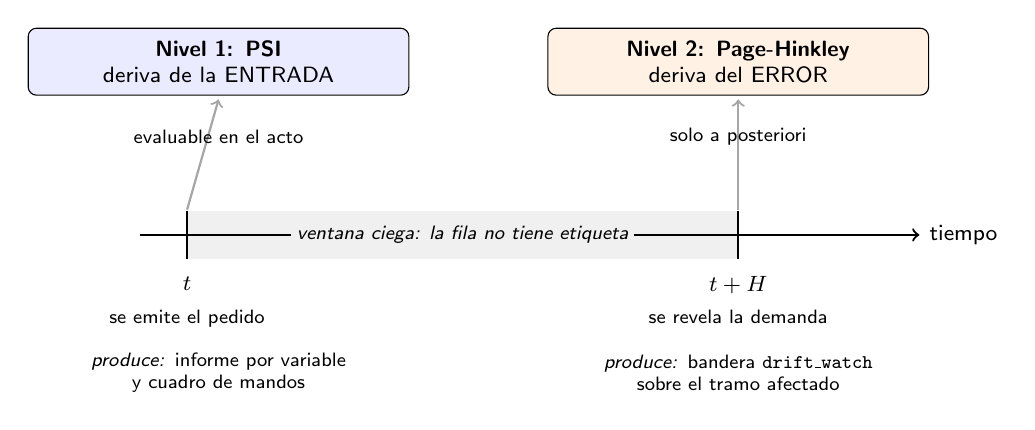
\begin{tikzpicture}[
    every node/.style={font=\sffamily\footnotesize, align=center},
    lvl/.style={draw, rounded corners=3pt, minimum height=0.85cm, text width=4.6cm},
    arr/.style={->, thick, gray!70},
    disp/.style={font=\sffamily\scriptsize, text width=4.6cm}
]
  % Franja de la ventana ciega y eje
  \fill[gray!12] (0,-0.3) rectangle (7,0.3);
  \draw[->, thick] (-0.6,0) -- (9.3,0) node[right, font=\sffamily\footnotesize] {tiempo};
  \draw[thick] (0,-0.3) -- (0,0.3);
  \draw[thick] (7,-0.3) -- (7,0.3);
  % Rotulo opaco para que el eje no lo atraviese
  \node[fill=gray!12, inner sep=2pt, font=\sffamily\scriptsize\itshape] at (3.5,0)
       {ventana ciega: la fila no tiene etiqueta};

  \node[below=3pt, font=\sffamily\footnotesize] at (0,-0.3) {$t$};
  \node[below=15pt, font=\sffamily\scriptsize] at (0,-0.3) {se emite el pedido};
  \node[below=3pt, font=\sffamily\footnotesize] at (7,-0.3) {$t+H$};
  \node[below=15pt, font=\sffamily\scriptsize] at (7,-0.3) {se revela la demanda};

  % Nivel 1: evaluable en el acto
  \node[lvl, fill=blue!8] at (0.4,2.2) {\textbf{Nivel 1: PSI}\\ deriva de la ENTRADA};
  \draw[arr] (0,0.32) -- (0.4,1.72);
  \node[disp] at (0.4,1.25) {evaluable en el acto};

  % Nivel 2: solo tras el horizonte
  \node[lvl, fill=orange!10] at (7.0,2.2) {\textbf{Nivel 2: Page-Hinkley}\\ deriva del ERROR};
  \draw[arr] (7,0.32) -- (7.0,1.72);
  \node[disp] at (7.0,1.25) {solo a posteriori};

  % Que produce cada uno
  \node[disp] at (0.4,-1.75) {\emph{produce:} informe por variable\\ y cuadro de mandos};
  \node[disp] at (7.0,-1.75) {\emph{produce:} bandera \texttt{drift\_watch}\\ sobre el tramo afectado};
\end{tikzpicture}
\shorthandon{>}%
\caption[Los dos niveles de monitorización]{Los dos niveles de monitorización, situados en el instante en que cada uno puede evaluarse. El nivel 1 compara distribuciones de entrada y no necesita esperar a nada; el nivel 2 mide el error y por tanto solo existe una vez transcurrido el horizonte. La franja sombreada es la ventana en la que el sistema ya ha decidido y todavía no puede saber si acertó, que es la limitación que la Sección~\ref{sec:contrato_operacional} enuncia como contrato. Ninguno de los dos promueve un reentrenamiento por sí solo.}
\label{fig:monitorizacion_niveles}
\end{figure}


\paragraph{Nivel 1: deriva de la distribución de entrada (PSI).} Vigila si las variables que alimentan al modelo siguen pareciéndose a aquellas sobre las que se ajustó. Es observable de inmediato, sin esperar a la demanda, y por eso es el nivel que puede operar en tiempo real. Para cada variable se calcula el \textit{Population Stability Index} entre una ventana de referencia y una ventana actual:

\begin{equation}
    \text{PSI} = \sum_{i=1}^{B} \left(p^{\text{act}}_i - p^{\text{ref}}_i\right) \ln \frac{p^{\text{act}}_i}{p^{\text{ref}}_i},
\end{equation}

donde $p^{\text{ref}}_i$ y $p^{\text{act}}_i$ son las proporciones de observaciones que caen en el intervalo $i$ de una discretización en $B = 10$ tramos. Los dos factores de cada sumando comparten siempre el signo, porque un tramo que gana masa tiene diferencia y logaritmo positivos y uno que la pierde los tiene ambos negativos, de modo que el índice es no negativo y se anula solo si las dos distribuciones coinciden. La expresión es, en esta forma simétrica, la divergencia de Jeffreys entre ambas distribuciones. Tres decisiones de cálculo condicionan la interpretación de la cifra. Primera, los bordes de los tramos son los \textbf{deciles de la distribución de referencia}, no una rejilla equiespaciada. Esta elección tiene una consecuencia que conviene explicitar porque simplifica la lectura del índice: por construcción cada tramo de referencia contiene una décima parte de las observaciones, es decir $p^{\text{ref}}_i \equiv 1/B$, y la ecuación se reduce a medir cuánto se aleja la distribución actual de repartirse por igual entre los deciles antiguos. El motivo de elegirlos es que sobre variables de demanda fuertemente asimétricas, una rejilla uniforme concentraría casi toda la masa en un tramo y el índice perdería resolución justo donde la tiene el fenómeno. Segunda, la ventana de referencia es la mitad \emph{más antigua} de las observaciones y la actual la mitad más reciente, con el corte en la fecha mediana: la deriva se mide así ``desde el entrenamiento'', que es la pregunta operativa. Tercera, el índice se reporta únicamente para las siete variables de mayor importancia según los valores SHAP del modelo explicado, porque una deriva en una variable que el modelo apenas usa no es un riesgo operativo sino ruido en el panel de alertas.

La lectura sigue las bandas convencionales del índice: por debajo de $0{,}10$ la distribución se considera estable, entre $0{,}10$ y $0{,}20$ hay un desplazamiento que merece seguimiento, y por encima de $0{,}20$ el desplazamiento es lo bastante grande como para cuestionar la validez del modelo ajustado.

\paragraph{Nivel 2: deriva del error del modelo (Page-Hinkley).} Vigila la magnitud que de verdad importa, si el modelo está empeorando, y por eso solo puede evaluarse a posteriori, cuando la demanda del horizonte se ha revelado. Se emplea una variante unilateral del contraste secuencial de Page-Hinkley sobre la serie de errores de validación: se acumula la desviación del error respecto a su media corriente, descontada una holgura $\delta$, y se declara deriva cuando esa acumulación excede su mínimo histórico en más de un umbral $\lambda$:

\begin{equation}
    m_T = \sum_{t=1}^{T}\left(e_t - \bar{e}_T - \delta\right),
    \qquad
    \text{PH}_T = m_T - \min_{t \leq T} m_t,
    \qquad
    \text{alerta si } \text{PH}_T > \lambda .
\end{equation}

Es \emph{unilateral} de forma deliberada: el contraste clásico detecta cambios de media en cualquier dirección, mientras que aquí solo interesa el error que \textbf{crece}. Una caída del error no es un incidente que haya que atender, y tratarla como tal llenaría el panel de alertas sin contenido accionable. En la configuración del sistema, $\delta = 0{,}005$ y $\lambda = 15$, y el estadístico se alimenta con el MAE de cada \textit{fold} del protocolo \textit{walk-forward}, de modo que lo que se vigila es la evolución del error a lo largo de la secuencia temporal de validación.

Ese mismo acoplamiento al protocolo acota lo que este nivel puede demostrar aquí, y conviene declararlo. Con $K = 3$ \textit{folds} el contraste recibe tres observaciones, y como exige un mínimo de dos antes de pronunciarse le queda una única oportunidad de disparo, en el último fold. En la corrida a escala el estadístico alcanza un máximo de $1{,}10$ frente a un umbral de $15$, un orden de magnitud por debajo, y no se emite ninguna alerta. El nivel 2 queda por tanto instrumentado y verificado, pero no ejercitado: un contraste secuencial necesita una secuencia, y la que este protocolo produce es demasiado corta para que la ausencia de alertas signifique nada sobre la estabilidad del modelo. Su lugar natural es el despliegue, donde los orígenes de decisión se suceden a diario y la serie de errores crece sin límite.

\paragraph{Qué dispara qué.} Conviene ser explícito sobre el alcance real de este subsistema, porque la distancia entre detectar y actuar es donde muchos sistemas de producción fallan silenciosamente. En el estado actual, \textbf{la detección informa y marca, pero no promueve por sí sola ningún reentrenamiento en caliente}: una alerta de Page-Hinkley marca las recomendaciones del tramo afectado con la bandera \texttt{drift\_watch} de la Sección~\ref{sec:excepciones} y queda registrada en la ejecución; el PSI por variable se persiste como informe y se sirve en el cuadro de mandos. El sistema contempla además la opción de forzar el reajuste del modelo en el \textit{fold} siguiente a una alerta, pero permanece desactivada en todas las configuraciones de este trabajo: un reentrenamiento disparado por deriva alteraría la política de actualización a mitad del protocolo y haría incomparables los \textit{folds} entre sí, precisamente la comparación que la simulación de cadencias de la sección siguiente necesita mantener limpia.

La decisión de cuándo reentrenar se toma, por tanto, por cadencia y no por alerta. Qué cadencia es la correcta no se resuelve por criterio sino midiéndola, y esa medición es el objeto de la sección siguiente.
\subsection{Elección Empírica de la Cadencia de Reentrenamiento}
\label{sec:simulate_ops}

La validación cruzada temporal (\textit{walk-forward backtesting}) estima el rendimiento del modelo en condiciones experimentales controladas. Sin embargo, en producción surge una pregunta adicional de naturaleza MLOps: \emph{\textquestiondown con qué frecuencia debe reentrenarse el modelo a medida que llegan datos nuevos?} Reentrenar demasiado frecuentemente supone un coste computacional elevado; hacerlo demasiado esporádicamente puede degradar las predicciones conforme el modelo queda desactualizado respecto a los patrones recientes.

Para responder esta pregunta de forma empírica sobre datos genuinamente no vistos, el sistema implementa una \textbf{Simulación Operacional en Streaming} sobre el split de evaluación. El esquema sigue el protocolo de \textbf{evaluación prequential} (\textit{interleaved test-then-train}), término acuñado por Dawid como contracción de \emph{predictive} y \emph{sequential} \cite{dawid1984prequential} y hoy estándar para evaluar aprendizaje sobre flujos de datos \cite{gama2013evaluating}. En lugar de partir los datos en conjuntos disjuntos, cada observación desempeña dos papeles en un orden fijo: primero sirve de prueba, porque el modelo la predice sin haberla visto, y solo después se incorpora al histórico disponible. De ahí que entrenamiento y prueba dejen de ser disjuntos sin que exista fuga alguna, y que el error pueda seguirse a lo largo del tiempo en vez de resumirse en una única cifra, que es justamente lo que un \textit{holdout} fijo no permite cuando la distribución se mueve. La variante que aquí se emplea difiere del esquema incremental clásico en un punto que constituye la propia variable del experimento: la observación entra en el histórico cada día, pero el modelo no se reajusta con ella hasta el siguiente reentrenamiento programado. El procedimiento es el siguiente:

\begin{enumerate}
    \item Se entrena un modelo \textit{champion} inicial exclusivamente sobre el split de entrenamiento. Este modelo representa el estado del sistema en el día de despliegue, antes de que llegue ningún dato del periodo de evaluación.
    \item Se define un conjunto de \textbf{cadencias de reentrenamiento}:
    \[K = \{k_1, k_2, \ldots, k_n, \text{nunca}\},\]
    donde cada $k_i$ es el número de días entre reentrenamientos consecutivos. El parámetro \texttt{simulation\_\allowbreak{}days} limita la ventana de evaluación. La cadencia \textit{nunca} sirve como \textit{baseline}: el modelo inicial nunca se actualiza.
    \item Se itera día a día sobre el split de evaluación, según el bucle que ilustra la Figura~\ref{fig:prequential_loop}. Para cada fecha de decisión $t$ y cada cadencia $k$:
    \begin{itemize}
        \item Se construye la \textbf{historia disponible} $\mathcal{H}_t = \text{train} \cup \text{eval}[\text{date} < t]$, garantizando ausencia de \textit{leakage}.
        \item Si $(t_{\text{index}} + 1) \bmod k = 0$, se reentrena el modelo de esa cadencia sobre $\mathcal{H}_t$, incluyendo recalibración conformal.
        \item El modelo genera predicciones para el horizonte $[t, t+H-1]$.
        \item Se revelan los datos reales del periodo y se calcula el coste de inventario realizado mediante el modelo Newsvendor.
    \end{itemize}
    \item Al finalizar el streaming, se dispone de curvas de \textbf{coste acumulado} por cadencia sobre el mismo periodo y los mismos datos, lo que permite una comparación directa y equitativa.
\end{enumerate}

\begin{figure}[H]
\centering
\shorthandoff{>}%
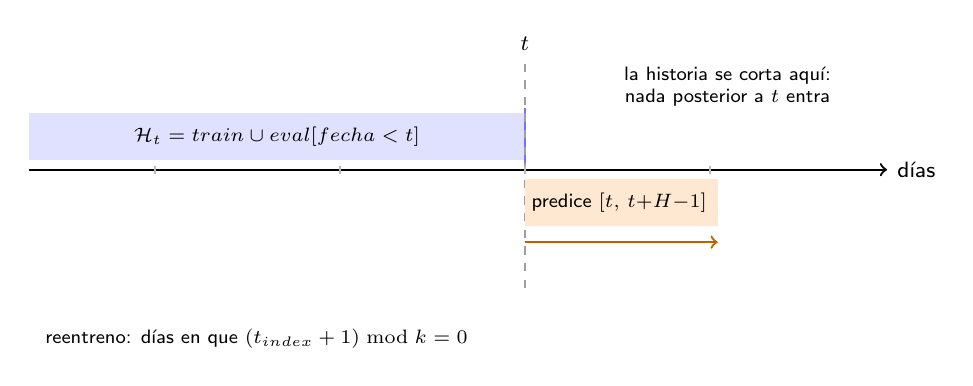
\begin{tikzpicture}[
    every node/.style={font=\sffamily\footnotesize, align=center},
    tick/.style={draw, thick, gray!55}
]
  % Eje de dias del split de evaluacion
  \draw[->, thick] (-0.3,0) -- (10.6,0) node[right, font=\sffamily\footnotesize] {días};

  % Historia disponible: se detiene ANTES de t
  \fill[blue!12] (-0.3,0.12) rectangle (6,0.72);
  \node[font=\sffamily\scriptsize] at (2.85,0.42)
       {$\mathcal{H}_t = \text{train} \cup \text{eval}[\text{fecha} < t]$};
  \draw[thick, blue!55] (6,0.08) -- (6,0.78);

  % Frontera de decision
  \draw[dashed, thick, gray!75] (6,-1.5) -- (6,1.35);
  \node[font=\sffamily\footnotesize] at (6,1.6) {$t$};

  % Horizonte de prediccion, hacia adelante
  \fill[orange!18] (6,-0.72) rectangle (8.45,-0.12);
  \node[font=\sffamily\scriptsize] at (7.2,-0.42) {predice $[t,\,t{+}H{-}1]$};
  \draw[->, thick, orange!75!black] (6,-0.92) -- (8.45,-0.92);

  % Reentrenos de la cadencia k
  \foreach \x in {1.3, 3.65, 6, 8.35} { \draw[tick] (\x,-0.05) -- (\x,0.05); }
  \foreach \x in {1.3, 3.65, 6, 8.35} {
      \node[font=\sffamily\scriptsize, gray!60!black] at (\x,-1.72) {$\blacktriangle$};
  }
  \node[font=\sffamily\scriptsize, anchor=west] at (-0.3,-2.15)
       {$\blacktriangle$ reentreno: días en que $(t_{\text{index}}+1) \bmod k = 0$};

  \node[font=\sffamily\scriptsize, anchor=west, text width=4.4cm] at (6.25,1.05)
       {la historia se corta aquí:\\ nada posterior a $t$ entra};
\end{tikzpicture}
\shorthandon{>}%
\caption[Un paso del bucle prequencial]{Un paso del bucle prequential para una cadencia $k$. En cada fecha de decisión $t$ el modelo solo ve la historia estrictamente anterior, predice hacia adelante el horizonte completo y se puntúa cuando esos días se revelan; el reentrenamiento se dispara cada $k$ días sobre la historia disponible en ese momento. El corte en $t$ es lo que hace que la comparación entre cadencias mida la política de actualización y no una fuga de información.}
\label{fig:prequential_loop}
\end{figure}

Esta simulación constituye la evidencia empírica que sostiene la política de reentrenamiento operacional del sistema.
